\documentclass{book}

\usepackage{float}
\usepackage{amsmath}
\usepackage{amsfonts}
\usepackage{graphicx}
\usepackage{lineno}
\usepackage{natbib}
\usepackage{hyperref}
\usepackage{verbatim}
\usepackage{soul}
\usepackage{color}

\bibliographystyle{asa}

\floatstyle{plain}
\floatname{panel}{Panel}
\newfloat{algorithm}{h}{txt}[chapter]
\newfloat{panel}{h}{txt}[chapter]


\newcommand{\R}{\textbf{R}}
\newcommand{\bugs}{\textbf{BUGS}}
\newcommand{\jags}{\textbf{JAGS}}
\newcommand{\secr}{\mbox{\tt secr}}
\newcommand{\scrbook}{\mbox{\tt scrbook}}


\linenumbers

\begin{document}


%\chapter{Introduction}
%\label{chapt.intro}

%\chapter{
Introduction to Spatial Capture-Recapture
}
\markboth{Introduction}{}
\label{chapt.intro}

\vspace{.3in}



Space: The final frontier. The spatial structure of populations, and
spatial processes that contribute to population dynamics,  
are central to  applied and theoretical population ecology.  At the
same time, the inherent spatial aspect of {\it sampling} populations
strongly affects apprent biases in how we observe population structure.
Books have been written on spatial processes in animals
oppulations \citep{tilman_kareiva:1997,hanski:1999}
and books have been written on how we sample these populations using
capture-recapture methods \citep{seber:1982,williams_etal:2003}.

Despite the central roll of space and spatial processes to both
understanding population dynamics and to how we observe population
structure, these two things have not yet been synthesized....... We do that
here, in this book.


Spatial processes structure animal populations --
-- movement, spatial variation in density, space usage, density dependence, interactions among individuals.
This is all about motive -- should not be about fixing technical
problems
with existing estimators but , rather, modeling actual ecological
processes.

SCR is about explicit formulations of CR models that involve space --
the spatial context of how we observe individuals , and what gives
rise to the distribution of individuals in space, and how individuals
use space, etc... 





\section{Capture-Recapture}

Information about abundance or density of populations, and their vital
rates, is fundamental to applied ecology and conservation biology.  To
that end, a huge variety of statistical methods have been devised, and
among these, the most well-developed are collectively known as
capture-recapture (or capture-mark-recapture) methods. For example,
the volumes by \citet{seber:1982}, \citet{borchers_etal:2002},
\citet{williams_etal:2002}, and \citet{amstrup_etal:2005} are largely
synthetic treatments of such methods, and contributions on modeling
and estimation using capture-recapture are plentiful in the
peer-reviewed ecology literature.  

Capture-recapture techniques have been the number 1 quantiative method
in studies of animal populations for decades.
But they apply basically to fish bowl sampling. Does it make sense
that methods should apply to both?

Capture-recapture techniques make
use of individual encounter history data, by which we mean sequences
of 0's and 1's denoting if an individual was encountered at a
particular trap during a certain time period. For example, the
encounter history ``010'' indicates that this individual was
encountered only during the second of three trapping occasions. As we
will see, these data contain
information about encounter probability, abundance, and other
parameters of interest in the study of population dynamics.

A diverse and growing number of methods exist for obtaining encounter
history data. Such methods are, naturally, taxa-specific. They include
classical ``traps'' which capture and retain animals until visited by
a biologist who removes the individual, marks it, or otherwise molests
it in some scientific fashion.  Small-mammal traps and mist nets for
birds are standard examples. Traps that physically capture and
restrain individuals are common, but capture-recapture methods no
longer require ``capture'' or even physical marking of individuals.
Recent technological advances have produced a
large number of passive detection devices that produce individual
encounter history data. These include camera traps
\citep{karanth_nichols:1998, oconnell_etal:2010}, acoustic recording
devices \citep{dawson_efford:2009}, and methods that obtain DNA
samples such as hair snares for bears \citep{gardner_etal:2010jwm}, scent
posts for many carnivores \citep{kery_etal:2010}, and related methods which allow DNA
to be extracted from scat, urine or animal tissue in order to identify
individuals.  This book is concerned with how such data can be used to
carry out inference about animal abundance or density, and other
demographic parameters such as survival, recruitment, and movement
using new classes of capture-recapture models which utilize auxiliary
spatial information related to the encounter process.  We refer to
such methods as spatial capture-recapture (SCR) models\footnote{In
the literature the term spatially explicit capture-recapture (SECR) is
also used}.

As the name implies, the primary feature of SCR models that
distinguishes them from traditional CR methods is that they make use
of the spatial information inherent to capture-recapture studies. That
is, the encounter histories are associated with spatial coordinates,
and these coordinates are informative about home range
characteristics, movement and space usage.
As we will see, this allows us to overcome three critical
deficiencies of non-spatial methods, namely,
traditional CR methods cannot be used to formally estimate density,
include of trap-level covariates of density or capture probability, or
account for heterogeneity in encounter probability that
results from the spatial organization of animals and traps.
Thus, spatial modeling is not just
a fun academic exercise; it provides a solution to basic problems in
the study of animal populations that have been acknowledged for more
than 70 years \citep{dice:1938}.
More important than just providing a resolution to
some basic technical problems,
SCR models provide
 a framework
for integrating
into capture-recapture models
explicit ecological hypotheses related to space usage,
and the spatial
organization of individuals in a population.
This greatly expands the practical utility and scientific
relevance of
capture-recapture methods and studies based on
encounter history data.

\section{Scope of this Book}

In this book, we try to achieve a broad methodological scope from
basic closed population models %using a number of distinct observation
%models
for inference about population density on up to open population models
for inference about vital rates such as survival and recruitment. %---spatial versions of
%conventional Jolly-Seber models. %A number of conceptual and
%methodological themes unify the main topical coverage of this book, and
%those are:
Much of the material is a synthesis of recent research but we also expand SCR models in a
number of useful directions, including to accomodate unmarked individuals
(Chapt. \ref{chapt.xxxx}), use of telemetry information (Chapt. \ref{chapt.rsf}), and developing
explicit models of individual space usage (Chapt. \ref{chapt.ecoldist}), and many other
new topics that have yet to appear in the literature.
Our intent is to
provide a comprehensive resource for ecologists interested in
understanding and applying SCR models to solve common problems
faced in the study of population dynamics. To do so, we make use of
hierarchical models, which allow extraordinary
flexibility in accommodating virtually any type of capture-recapture
data. We present many example analyses, of real and simulated data
using likelihood-based and Bayesian methods---examples that readers
can replicate using the code presented in the text and
the resources made available on-line and in our accompanying {\bf R} package
{\tt scrbook}.

Although we aim to reach a
broad audience, at times we go into details that may only be of
interest to advanced practitioners who need to extend these models to
unique situations.  We hope that these advanced topics will not
discourage those new to these methods, but instead we believe this
material will allow readers to advance their understanding and become
less reliant on restrictive tools and software. Before discussing the
specifics of SCR models, we begin with an overview of the methods
used to collect capture-recapture data, and provide a brief summary of
traditional non-spatial capture-recapture models.



In this book we present a diverse array of modeling approaches for making
inference about density and population dynamics using spatial
capture-recapture data. A number of conceptual and
methodological themes unify the main topical coverage of this book, and
those are:

\begin{itemize}
\item[(1)] Hierarchical modeling. We develop hierarchical models
  consisting of explicit models for both the observation process and
  the underlying ``ecological process'' which describes the
  organization of individuals in space.

\item[(2)] Formal inference using both classical (frequentist,
  likelihood-based) and Bayesian methods. We often emphasize
  Bayesian analysis because this allows us to focus the technical
  formulation of models, and spatial capture-recapture is mainly
  concerned with modeling random effects and estimating functions of
  random effects. However, we also explore likelihood methods using existing
  software such as the R package SECR \citep{efford:2011}, as well as
  development of custom solutions along the way.

\item[(3)] In developing Bayesian analyses of SCR models, we emphasize
  the use of the BUGS language for describing models. The BUGS
  language emphasizes the syntactic description of the essential
  assumptions of models in a special kind of pseudo-code language,
  which is used in software (WinBUGS, JAGS, OpenBUGS) to devise Markov
  chain Monte Carlo (MCMC) algorithms for Bayesian analysis of
  models. The BUGS language focuses your thinking on model development
  and lets you develop an understanding of models at the level of
  their basic assumptions and structure.  Despite our focus on
  describing models using the BUGS language, we also show readers how
  to devise their own MCMC algorithms for Bayesian analysis of SCR
  models, which can be convenient (even necessary) in some practical
  situations.

\item[(4)] Data augmentation -- dealing with the fact that population
  size, $N$, is unknown is a challenging technical problem in
  capture-recapture models. We confront this problem in almost every
  chapter of this book. To deal with it we use a technical device
  called {\it data augmentation} which is extremely useful for
  analysis of capture-recapture models that are specified
  ``conditional on $N$'' \citep{royle_etal:2007}.
\end{itemize}

Altogether, these different conceptual and methodological elements
provide for a formulation of SCR models that essentially renders them
as variations of generalized linear mixed models (GLMMs). This in a
sense makes them consistent with many important methodologies used in
ecology (e.g., see \citet{zuur_etal:2009, kery_etal:2010}), and
because of the connection with standard modeling concepts, we believe
that the material presented in this book can be understood and used by
most ecologists with some modeling experience.

This book is not a book about Bayesian analysis, not a book about
hierarchical models, not a book about capture-recapture, and not about
programming in R. In a sense though, our book integrates elements of
all of these things into what we hope is a coherent package for
analyzing data from this enormous class of data collection methods
that produce spatially-explicit capture-recapture data.   As such, we
expect that people have a basic understanding of statistical models
and classical inference (What is frequentist inference? what is a
likelihood? Generalized linear model? Generalized linear mixed
model?),
{\bf R} programming,
 Bayesian analysis (what is s a prior distribution and a
posterior distribution?),
and maybe even a little bit
of Bayesian
computation (MCMC and perhaps the BUGS language).
The ideal candidate for reading this book has basic knowledge of these
topics. However, we do provide introductory chapters on the necessary
components which we hope can serve as a brief and cursory tutorial for
those who might have only limited technical knowledge, e.g., many
carnivore biologists who implement field sampling programs but do not
have extensive experience analyzing data.



\section{Lions and Tigers and Bears, oh my:  Genesis of
Spatial capture-recapture data}

A diverse number of methods and devices exist for producing individual
encounter history data with auxiliary spatial information about
individual locations. Historically, physical ``traps'' have been widely
used to sample animal populations. These include live traps, leg-hold
traps, mist nets, pitfall traps and many other types of
devices. Although these are still widely used, 
recent technological advances 
for obtaining encounter history
data non-invasively 
 have made it possible to study many species that
were difficult if not impossible to study effectively just a few years
ago.  And, 
 we believe, these methods have revolutionized the study of animal populations by
 capture-recapture methods and will lead to their increasing
 relevance in the future.
 We briefly review some of these here, which we
 consider more explicitly in later chapters of this book.

\subsection{Camera trapping}

Considerable recent work has gone into the development of
camera-trapping methodologies. For a historical overview of this
method see \citet{kays_etal:2008} and \citet{kucera_barrett:2011}.  Several
recent synthetic works have been published including
\citet{nichols_karanth:2002}, and an edited volume by
\citet{oconnell_etal:2010} devoted solely to camera trapping concepts
and methods. As a method for estimating abundance, some of the earliest
work that relates to the use of camera trapping data in
capture-recapture models originates from Karanth and colleagues
\citep{karanth:1995, karanth_nichols:1998, karanth_nichols:2000}. In
camera trapping studies, cameras are situated along trails or
at baited stations and individual animals are photographed and
subsequently identified either manually by a person sitting behind a
computer,  or sometimes now using computational
methods. Camera trapping methods are widely used for species that have
unique stripe or spotting patterns such as tigers \citep{karanth:1995,
  karanth_nichols:1998}, ocelots
\citep{trolle_kery:2003,trolle_kery:2005}, leopards
\citep{balme_etal:2010}, and many other cat species.
% Scientific names
Camera traps are
also used for other species such as wolverines 
\citep[{\it Gulo gulo}][]{magoun_etal:2011,royle_etal:2011}, 
and even species that are less easy to
identify uniquely such as mountain lions \citep{sollmann_etal:inprep} 
and coyotes  %add scientific names
(e.g. \citet{kelly_etal:2008}.  We note that even for species that are
not readily identified by pelage patterns, it might be efficient to use
camera traps in conjunction with spatial capture-recapture models to
estimate density (see Chapt.~\ref{chapt.scr-unmarked}).
%, if an initial sample of individuals can be collared
%or tagged in some way so that subsequent encounter by camera-traps can
%yield individual information. In this way, the probability of
%encounter can be estimated from the camera traps based on the
%pre-marked individuals, and this is applied to the frequencies of
%unmarked individuals to estimate density.


\begin{figure}
\begin{center}
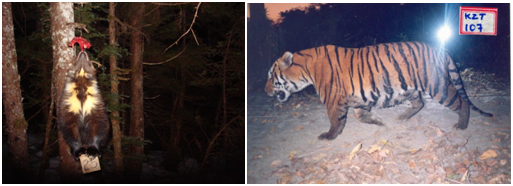
\includegraphics[width=5in]{Ch1/figs/wolverinetiger}
\end{center}
\caption{
Left: Wolverine being encounter by a
camera trap ({\it Photo credit: Audrey Magoun}).
Right: Tiger encountered by
camera trap ({\it Photo credit: Ullas Karanth/WCS}).
}
\label{fig.wolverinetiger}
\end{figure}

\subsection{DNA Sampling}

DNA obtained from hair, blood or scat is now
routinely used to obtain individual identity and encounter history
information about individuals \citep{taberlet_bouvent:1992,
  woods_etal:1999, mills_etal:2000, schwartz_monfort:2008}.  A common
method is based on the use of ``hair snares'' (Fig. \ref{fig.bearcat})
which are widely used to study bear populations
\citep{woods_etal:1999, gardner_etal:2010jwm, garshelis_etal:2006,
  kendall_etal:2009}.  A sample of hair is obtained as individuals
pass under or around barbed-wire (or other physical mechanism) to take
bait. Hair snares and scent sticks have also been used to sample felid populations
\citep{garciaalaniz_etal:2010, kery_etal:2010} and other species. Research has even shown that
DNA information can be extracted from urine deposited in the wild (e.g., in snow; see \cite{valiere_taberlet:2000})
and as a result this may prove another future data collection technique where SCR models
are useful.

\begin{figure}
\begin{center}
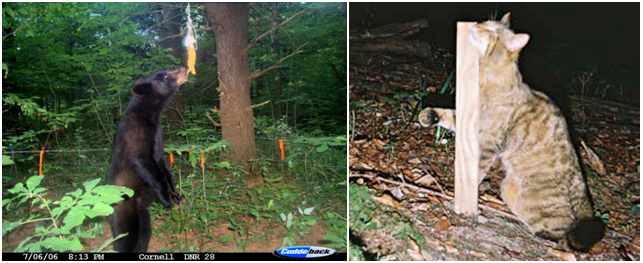
\includegraphics[width=5in]{Ch1/figs/bearcat}
\end{center}
\caption{Left:  Black bear in a hair snare ({\it Photo credit: M. Wegan})
Right: European wildcat loving on a scent stick ({\it Photo credit: Darius
Weber, Hintermann \& Weber AG, Ecological Consultancy, Planning \&
Research, Switzerland})
}
\label{fig.bearcat}
\end{figure}


\begin{figure}
\begin{center}
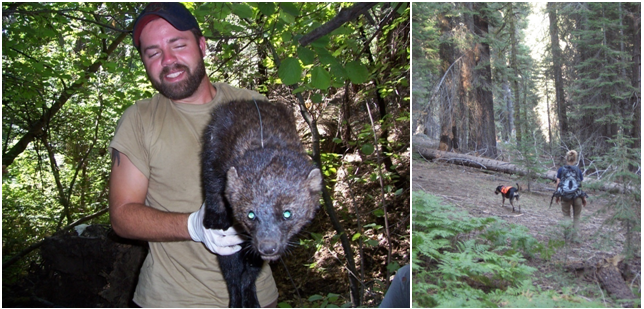
\includegraphics[width=5in]{Ch1/figs/beardog}
\end{center}
\caption{Left:
A wildlife research technician for the USDA Forest Service
  holding a male fisher  captured as part of the Kings River Fisher
  Project in the Sierra National Forest, California.
Right: A dog handler surveying for fisher scat in the Sierra National Forest.
{\it Photo credit: Craig Thompson, USDA Forest Service,
Pacific Southwest Research Station.}}
\label{fig.fisherscatdog}
\end{figure}


\subsection{Acoustic surveys}

Many studies of birds \citep{dawson_efford:2009}, bats, and whales \citep{marques_etal:2009}  now collect data using
devices that record vocalizations. When vocalizations can be identified by individual from multiple
recording devices, spatial encounter histories are produced that are amenable to
the application of SCR models \citep{dawson_efford:2009, efford_etal:2009ecol}.

\subsection{Search-Encounter Methods}

There are other methods which don't fall into a nice clean taxonomy of
``devices''. Spatial encounter histories\footnote{defined? probably
  not! need to do that} are commonly obtained by conducting manual
searches of geographic sample units such as quadrats, transects or
road or trail networks.
For example,
DNA-based encounter histories can be obtained from scat
samples located along roads or trails or by specially trained dogs
\citep{mackay_etal:2008} searching space
(Fig. \ref{fig.fisherscatdog}). This method has been used in studies
of martens, fishers \citep{thompson_etal:inpress}, lynx, coyotes,
birds \citet{kery_etal:2010}, and many other species. We might search
space on foot and pick up individuals and physically mark them
somehow. This is pretty common in surveys that involve reptiles and
amphibians, e.g., we might walk transects picking up 
box turtles \citep{hall_etal:1999}, or desert tortoises \citep{zylstra_eta:2010},
 or search space for lizards
\citep{royle_young:2008} and also surveys designed to obtain animal
scat. These methods don't seem like normal capture-recapture in the
sense that the encounter of individuals is not associated with
specific trap location, but SCR models are equally relevant for
analysis of such data (see Chapt. \ref{chapt.searchencounter}).


\section{ Historical Context: A Brief Synopsis of the Literature}

Spatial capture-recapture is a relatively new methodological
development, at least with regard to formal estimation and
inference. However, the basic problems that motivate the need for
formal spatially-explicit models have been recognized for decades and
quite a large number of ideas have been proposed to deal with these
problems. We review some of these ideas here.


\subsection{Buffering}

 The standard approach to estimating density even now is to estimate $N$ using
conventional closed population models \citep{otis_etal:1978} and then
try to associate with this estimate some specific sampled area, say $A$,
the area which is contributing individuals to the population for which
$N$ is being estimated. The strategy is to define $A$ by placing a buffer
of say $W$ around the trap array or some polygon which encloses the trap
array. The historical context is succinctly stated by \citep{obrien:2011}
from which we draw this description:

\begin{quote}
  ``At its most simplistic, $A$ may be described by a concave polygon
  defined by connecting the outermost trap locations ($A_{tp}$; \citet{mohr:1947}).
 This assumes that animals do not move from outside the
  bounded area to inside the area or vice versa. Unless the study is
  conducted on a small island or a physical barrier is erected in the
  study area to limit movement of animals, this assumption is unlikely
  to be true. More often, a boundary area of width $W$ ($A_{w}$) is added to
  the area defined by the polygon $A_{tp}$ to reflect the area beyond the
  limit of the traps that potentially is contributing animals to the
  abundance estimate \citep{otis_etal:1978}. The sampled area, also known
  as the effective area, is then $A(W) = A_{tp} + A_{w}$. Calculation of the
  buffer strip width ($W$) is critical to the estimation of density and
  is problematic because there is no agreed upon method of estimating
  $W$. Solutions to this problem all involve ad hoc methods that date
  back to early attempts to estimate abundance and home ranges based
  on trapping grids
  \citep[see][]{hayne:1949}. \citet{dice:1938} first drew attention
  to this problem in small mammal studies and recommended using
  one-half the diameter of an average home range. Other solutions have
  included use of inter-trap distances \citep{blair:1940,burt:1943}, mean
  movements among traps, maximum movements among traps \citep{holdenried:1940, hayne:1949},
 nested grids \citep{otis_etal:1978}, and assessment
  lines \citep{smith_etal:1971}.''
\end{quote}

The idea of using 1/2 mean maximum distance moved
\citep{wilson_anderson:1985a} seems to be the standard approach even
today, presumably justified by Dice's suggestion to use 1/2 the home
range diameter. Alternatively, some studies have used the full
MMDM (e.g. \citet{parmenter_etal:2003}),

%\footnote{Do they really say that?}  Yes, they really do use it, but so
%do a lot of studies so we can add more if you want.

because the trap array might not provide a full coverage of the home range so 1/2 MMDM may be smaller than the home range radius. And, sometimes home range size is
estimated by telemetry \citep{karanth:1995, bales_etal:2005}.
%\footnote{Is this correct cite for this?}.  Karanth used some technique, it's hard to tell for sure....but he
% mentions using 1 female that is collared to estimate effective trap area.  Bales does it too, so I added it for
% extra value!

This is usually combined
with an AIC-based selection from among the closed-population models in
\citet{otis_etal:1978} which most often suggests heterogeneity in detection (Model
Mh).  Almost all of these early methods were motivated by studies of
small mammals using classical ``trapping grids'' but, more recently,
their popularity has increased with the advent of new technologies and
especially related to non-invasive sampling methods such as camera
trapping. In particular, the series of papers by Karanth and Nichols
\citep{karanth:1995, karanth_nichols:1998, karanth_nichols:2002}
has led to fairly widespread adoption of these ideas.

Some of the heuristic ideas based on buffer strips do have some
technical justification in the sense of estimating parameters of an
underlying movement model from observed movements. For example, if we
let $x$ be a random variable indicating movement outcomes of an
individual about its  home range center, and suppose that $x$ has pdf
$g(x)$ then we can understand properties of MMDM by studying the
properties of the sample order statistics, as the maximum distance
moved is the sample range based on a sample of observations of
individual locations.



%As an illustration, imagine a 1-dimensional
%system where individuals have a home range that amounts to a line
%segment. Then suppose that individual movements are $\mbox{uniform}(0,A)$. It
%can be shown that the sampling distribution of the sample range, R,
%scaled by $A$, say $R/A$ has a beta distribution, $\mbox{beta}(n-1,2)$
%\citep[][p. 235]{casella_berger:2002}
%and thus the diameter of the home range, i.e. $A$, is
%estimated (biasedly) by$ R/( (n-1)/(n+1) )$. For large $n$ we could then
%say that the sample range, i.e., ''maximum distance moved'' seems like a good estimator of home range diameter and, therefore, $R/2$ is an estimator of home-range radius.

%There are a number of technical issues that arise in attempting to use
%such heuristics to justify the application in practice. For one, the
%moments of the sample order statistics are strongly affected by sample
%size, which is typically quite small (per individual encountered) and
%thus, in general, are biased and estimated with variable precision
%depending on sample size. For example, the expected value of MMDM is
%$k(n)*A$ , i.e., the true home range diameter is related to observed
%MMDM by some function of sample size, $k(n)$, that increases to 1. In
%the case where the underlying movement model is uniform, $k(n) =
%(n-1)/(n+1)$ (from above) which motivates a formula for ``adjusting''
%observed MMDM for small sample size. We suspect that many such
%formulae are obtainable depending on the assumed movement distribution
%\citep[e.g., formula 6.16 in][]{obrien:2011}. We might also think about taking
%the {\it maximum} (over individuals) of the maximum distance moved
%because under the specific model considered here (iid uniform) then
%all individuals have the same home range radius. This increases our
%sample size ($n$) and thus the observed sample range should be more
%accurate.


%%Another issue of somewhat more importance (and less easy to
%rectify) is that the {\it observation} of movement outcomes is biased
%by the locations of traps. We cannot observe movements ``off the
%trapping grid'' (or between traps) and thus our observed movements
%will generally be smaller than expected under any particular model
%(the uniform in this case). Moreover, the trap spacing also induces a
%discreteness to the movements that causes a further level of
%approximation based on hypothetical movement
%distributions. Nevertheless, formal analysis of `` buffering''
%strategies based on sample order statistics under specific models for
%movement does at least provide some heuristic support for specific
%choices.  The interested reader should ponder the distribution of the
%sample minimum, maximum and range under other distributions such as a
%normal (and bivariate normal), exponential distribution and perhaps
%others. In addition, contemplate the effect of censoring of movements
%to some arbitrary limit ($B<A$) to mimic bias in observed movement
%outcomes due to a finite trap grid.

\subsection{Trapping webs}

The use of buffer strips is conventional and widespread due to the
heuristic appeal of that idea and its easy implementation, but other
conceptual approaches exist to address specific problems motivated by
the spatial context of capture-recapture data. D.R. Anderson came up
with the idea of the ``trapping web'' \citep{anderson_etal:1983} which
does not seem to have been widely adopted in practice.
% although there
%is a clear mathematical formalization to the trapping web design
%\citep{link_barker:1994}.
One reason for this is
the design is somewhat restrictive in the sense that it requires
a large number of traps be organized in close proximity to one
another.

\subsection{Temporary Emigration}

Another intuitively appealing idea is that by \citet{white_shenk:2000}
who discuss ``correcting bias of grid trapping estimates'' by
recognizing that the basic problem is like random temporary emigration
\citep{kendall_etal:1997} where individuals flip a coin with
probability $\phi$ to determine if they are ``available'' to be
sampled or not.  White and Shenk's idea was to estimate $\phi$ from
radio telemetry, as the proportion of time an individual spends in the
study area. They obtain the estimated super-population size by using
standard closed population models and then obtain density by $\hat{D}
= \hat{N}\hat{\phi}/A$ where $A$ is the nominal area of the trapping
array (e.g., minimum convex hull).  A problem with this approach is
that individuals that were radio collared represent a biased sample
i.e., you fundamentally have to sample individuals randomly from the
population {\it in proportion to their exposure to sampling} and that
seems practically impossible to accomplish. In other words, ``in the study area'' has no
precise meaning itself and is impossible to characterize in almost all capture-recapture studies.
Deciding what is ``in the study area'' is effectively the same as choosing an arbitrary buffer which defines
who is in the study area who who isn't.
That said, the temporary
emigration analogy is a good heuristic for understanding SCR models
and has a precise technical relevance to certain models.

Another very interesting idea is that of using some summary of
``average location'' as an individual covariate in standard
capture-recapture models. \citet{boulanger_mclellan:2001} use
distance-to-edge (DTE) as a covariate in the Huggins-Alho type of
model. \citet{ivan:2012} uses this approach in conjunction with an
adjustment to the estimated $N$ obtained by estimating the proportion of
time individuals are ``on the area formally covered by the grid''
using radio telemetry.  We do not dwell too much on these different
variations but we do note that the use of DTE as an individual
covariate amounts to some kind of intermediate model between simple
closed population models and fully spatial capture-recapture models,
which we address directly in Chapt. \ref{chapt.closed}.
%We note that no adjustment
%based on telemetry information is necessary if one were simply to
%place a prior distribution on the individual covariate (which is not
%to say that telemetry data isn't useful, just that the same objective
%can be achieved without telemetry data).

While these procedures are all heuristically appealing, they are also
essentially ad hoc in the sense that the underlying model remains
unspecified or at least imprecisely characterized and so there is
little or no basis for modifying, extending or generalizing the
methods. These methods are distinctly {\it not} model-based procedures
even though they might well be heuristically appealing under specific
movement models. Despite this, there seems to be an enormous amount of
literature developing, evaluating and ``validating'' these literally
dozens of heuristic ideas that solve specific problems, as well as
various related tweeks and tunings of them and really it hasn't led to
any substantive breakthroughs that are sufficiently general or
theoretically rigorous.



%A classical argument in favor of the HA model is
%that it ``doesn't require assumptions about the covariate'' but the
%assumption is explicit in capture-recapture models and thus it is
%natural to attack inference based on the ``joint likelihood''
%\citep{borchers_etal:2002}. This has proven necessary in certain other
%classes of individual covariate models in which natural models arise
%for the individual covariate, such as time-varying individual
%covariates \citep{bonner_schwarz:2006}, or covariates with measurement
%error (e.g., distance sampling; see
%\citet[][ch. 7]{royle_dorazio:2008}).
%The model-based formulation is easily adapted to standard
%individual covariate models as well \citep{royle:2008}. Throughout
%this book we rely heavily on Bayesian inference of the joint
%likelihood, using the formulation based on data-augmentation
%\citep{royle_etal:2007, royle_young:2008, royle:2009} though we also
%discuss the development of likelihood-based inference in chapter 5 and
%apply those methods in some cases.


\section{The Failure of Classical Capture-Recapture}

XXXX Motive should probably go here , or immediately in next
section XXXXXXX


We briefly introduced and reviewed a number of classical techniques for applying non-spatial capture-recapture
models to studies of animal populations. These techniques, such as buffering, are based on many heuristically appealing
ideas.
But these are just heuristics and do not resolve the essential, basic problem with conventional
(''non-spatial'') capture-recapture models which is that there is no linkage {\it in the model} between
the quantity being informed by the data (i.e., $N$) and any stated or prescribed ``area'', $A$.

More generally,
ordinary capture-recapture methods are
distinctly non-spatial. They don't admit spatial indexing of either sampling
(the observation process) or
of individuals (the ecological process). This leads immediately to 3 main deficiencies:
 (1)
Ordinary CR models do not provide a coherent basis for estimating density.
For capture-recapture models to provide a coherent framework for inference about population density,
$N$ has to scale, as part of the model, with $A$ so that the model imposes biological context
on $A$ (i.e., as the area over which the $N$ individuals reside). SCR models achieve this.
(2) Ordinary CR models {\it induce} a form of heterogeneity that can
 only at best be approximated by classical models of latent heterogeneity. SCR models formally
 accommodate heterogeneity due to the juxtaposition of individuals with the encounter devices.
(3) Ordinary CR models do not accommodate trap-level covariates which
 exist in a large proportion of real studies. Again, SCR models formally
 accommodate heterogeneity due trap variation.  %or something like that last sentence
 %so that all 3 issues match.


Here we confront some of the issues that motivate the need for spatial
capture-recapture models by considering analysis of data from a study
design to estimate black bear abundance on the Fort Drum Military
Installation in upstate New York (see Chapt. \ref{chapt.closed} for more details). The
specific data used here are encounter histories on 47 individuals
obtained from an array of 38 baited ``hair snares'' during June and
July 2006. The study area and locations of the 38 hair snares are
shown in Fig. \ref{fig.hairsnares}.  Barbed wire traps (see
Fig. \ref{fig.bearcat}) were baited and checked for hair samples each
week for eight weeks.  Analysis of these data appears in
\citet{gardner_etal:2010jwm} and we use the data in a number of analyses
in later chapters.

\begin{figure}
\begin{center}
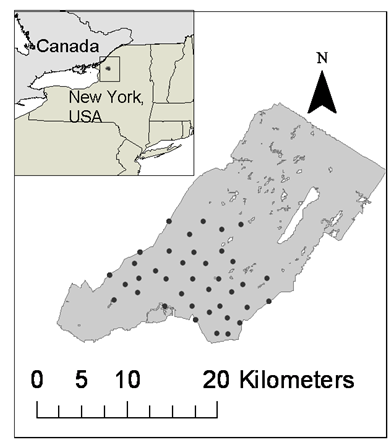
\includegraphics[height=3in]{Ch1/figs/hairsnares}
\end{center}
\caption{Locations of black bear hair snares on Fort Drum.}
\label{fig.hairsnares}
\end{figure}

We regarded this data set as a standard capture-recapture data set -
an encounter history matrix with 47 rows and 8 columns with entries
$y_{ik}$, where $y_{ik}=1$ if individual $i$ was captured in sample
$k$ and $y_{ik}=0$ otherwise. There is a standard closed population
model, colloquially referred to as ``model $M_0$'' (see Chapt. \ref{chapt.closed}), which
assumes that encounter probability $p$ is constant for all individuals
and sample periods.  We fitted model $M_0$ to the Fort Drum data using
traditional likelihood methods, yielding the maximum likelihood
estimate (MLE) of $\hat{N} = 49.19$ with an asymptotic standard error
(SE) of $1.9$.

The key issue in using closed population models with such data is how
on earth do we interpret this estimate of $N=49.19$ bears? Does it
represent the entire population of Fort Drum? Certainly not -- the trapping array covers less than
half of Fort Drum! (Fig. \ref{fig.hairsnares}). So to get at the total bear
population size of Fort Drum, we'd have to convert our $\hat{N}$ to
an estimate of density and extrapolate. To get at density, then,
should we
assert that $N$ applies to the southern half of Fort Drum below some
arbitrary line? Surely bears move on and off of Fort Drum without
regard to hypothetical boundaries. Without additional information
there is simply no way of converting this estimate of $N$ to density,
and hence it is really not meaningful biologically. To resolve this
problem, we will adopt the customary approach of converting $N$ to $D$
by buffering the convex hull around the trap array. The convex hull
has area $157.135$ $km^2$. We follow \citet{bales_etal:2005} in
buffering the convex hull of the trap array by the radius of the mean
female home range size.


%%%%\footnote{Did Bales et al. actually do this?}.
%HERE IS WHAT BALES DID:  First, we created a 95% minimum convex polygon
%for all radiolocations of adult females used in homerange
%analyses (Figure 1). Second,we buffered the
%100% minimum convex polygon for trapping locations
%with the approximate radius of the average
%95% minimum convex polygon home range of adult
%females (n = 13) using ArcView (ESRI, Redlands,
%Calif.).


The mean female home range radius was
estimated \citep{wegan:2008} for our study region to be $2.19$
km,
%\footnote{Is this number right out of Wegan's disseration?}
% YES, this is straight out of his thesis.
and
the area of the convex hull buffered by $2.19$ km is $277.01$
km$^2$. ({\bf R}
commands to compute the convex hull, buffer it, and compute the area
are given in the {\bf R} package \mbox{scrbook} which accompanies the
book).  Hence, the estimated density
here is approximately $0.178$ bears/km$^2$ for an estimated population
size obtained using model $M_0$.  We could assert that the problem has
been solved, go home, and have a beer.  But then, on the other hand,
maybe we should question the use of the estimated home range radius
 -- after all, this is only the female home range radius and the home ranges
 change for many reasons. Instead, we may decide to rely on a buffer width based on
one-half MMDM estimated from the actual hair snare data as is more customary
\citep{dice:1938}. In that case the buffer width is $1.19$ km, and the
resulting estimated density is increased to $0.225$ bears/ha$^2$ about
27 \% larger.  But wait - some studies actually found the full MMDM
\citep{parmenter_etal:2003} to be a more appropriate measure of
movement (e.g \citet{soisalo_cavalcanti:2006}). So maybe we should use
the full MMDM
which is $2.37$ km, pretty close to the telemetry-based estimate
and therefore providing a similar estimate of density ($0.171$
bears/ha$^2$). So in trying to decide how to buffer our trap array we
have already generated 3 density estimates. The crux of the matter is
obvious: Although it is intuitive that $N$ should scale with area --
the number of bears should go up as area increases and go down as area
decreases -- in this ad hoc approach of accounting for animal movement
$N$ remains the same, no matter what area we decide we sampled. The
number of bears and the area they live in are not formally tied
together within the model, because estimating $N$ and estimating the
area $N$ refers to are two completely independent analytical steps which are unrelated to one another by a
formal model.

Unfortunately, our problems don't end here. In thinking about the use of model $M_0$, we might naturally question
some of the basic assumptions that go into that model. The obvious one
to question is that which declares that $p$ is constant. One obvious
source of variation in $p$ is variation {\it among individuals}. We
expect that individuals may have more or less exposure to trapping due
to their location relative to traps, and so we try to model this ``heterogeneous''
encounter probability
phenomenon.
To illustrate this here are the number of traps that each individual was captured in:
\begin{verbatim}
 #traps:  1   2  3  4  5  6  9
 #bears: 23  13  6  2  1  1  1
\end{verbatim}
suggesting quite a range in traps exposed to by different bears.
%%% #bears: 19 15  5  2  2  1  1  1  1
% But, being captured in different numbers of traps is {\it not} inconsistent with a non-spatial model.
%That is if individuals roamed randomly over space with no ``home range'' then you should expect them to be captured
%in varying numbers of traps also.....
This has led many to consider
capture-recapture models that allow for individual heterogeneity in
$p$. Such models have the colloquial name of ``model $M_h$.''
We fitted this model (see Chapt. \ref{chapt.closed} for details) to the Fort Drum data
using each of the 3 buffer widths previously described (telemetry, 1/2
MMDM and MMDM), producing the estimates reported in Table
\ref{intro.tab.fdests}. While we can tell by the models' AIC that $M_h$ is
clearly favored by more than 30 units, we might still not be entirely
happy with our results. Clearly there is information in our data that
could tell us something about the exposure of individual bears to the
trap array -- where they were captured, and how many times -- but
since space has no representation in our model, we can't make use of
this information. Model Mh thus merely accounts for what we observe in
our data (some bears were more frequently captured than others) rather
than explicitly accounting for the processes that generated the data.

So what are we left with?  Our density estimates span  a range
from $0.17$ to $0.43$ bears/km$^2$ depending on which estimator of $N$ we use and
what buffer strip we apply. Should we feel strongly about one or the other?
Which buffer should we prefer?
AIC favors model $M_h$, but did it adequately account for the differences in
exposure of individuals to the trap array? Are we happy with a purely phenomenological model
for heterogeneity? One that posits that all bears are $iid$ draws from some distribution?
It assumes that all individuals are iid draws from some distribution but does not
account for the explicit mechanism of induced heterogeneity. And, further, we have information
about that (trap of capture) which model Mh ignores.
%Moreover, we could find more variations of
%model Mh to choose among, but see \citep{link:2003}.
And if we choose one type of buffer, how do we compare our density estimates
to those from other studies that may opt for a different kind of buffer?
The fact that $N$ doesn't scale with $A$, as part of the model, renders this choice
arbitrary. The buffer isn't part of the model.
\begin{comment} So
how do we characterize uncertainty of the buffer ``estimate''?  And,
in what sense is the
buffer even an estimate of something? What is it an estimate of?
\end{comment}
Clearly,
there is not a compelling solution to be derived from
this ``estimate $N$ and conjure up a buffer'' approach
and we are left not much wiser about bear density at
Fort Drum than we were before we conducted this analysis.

%%%% We could just finish this part off with a paragraph about these additional open questions -
%%%%the whipped cream of problems on the capture-recapture sundae - including the trap-level covariates;
%%%%or we could come up with some trap-level covariate example for the bears (different baits used, blabla).
\begin{comment}
Some of the open questions at this point:
How do we characterize uncertainty of the buffer ``estimate''?  And,
in what sense is the
buffer even an estimate of something? What is it an estimate of?
The summary here should be that there's not a compelling solution to be derived from
this ``estimate $N$ conjure up a buffer'' approach.
{\bf The main point that N doesn't scale with A is not made
  clearly here.}
\end{comment}


\begin{table}[ht]
\centering
\caption{Table on estimates of D for the Fort Drum data
using models $M_0$ and $M_h$ and different buffers. Model $M_h$ here
is a logit-normal mixture \citep{coull_agresti:1999}.}
\begin{tabular}{ll|cc}
\hline
model & buffer &  $\hat{D}$ & SE \\ \hline
M0   & telemetry &  0.178 & 0.178 \\
M0    & MMDM     &  0.171 & 0.171\\
M0   & 1/2 MMDM  &  0.225 & 0.225\\
Mh(ln) & telemetry &0.341 & 0.144\\
Mh(ln) & MMDM    &  0.327 & 0.138\\
Mh(ln) & 1/2 MMDM & 0.432 & 0.183\\
\end{tabular}
\label{intro.tab.fdests}
\end{table}


\section{Extension of Closed Population Models}
XXX Spatial context of populations ?? XXXXXX


The deficiency with classical closed population models is that they
have no spatial context. $N$ is just an integer parameter that applies
equally well to some population that exists in a computer, estimating the number
of unique words in a book, or a bucket full of goldfish.  The question
of {\it where} the $N$ items belong is central both to interpretation
of data and estimates from all capture-recapture studies and, in fact,
to the construction of spatial capture-recapture models considered in
this book.  Surely it must matter whether the $N$ items exist as words
in a book, or goldfish in a bowl, or birds in a forest patch! That
classical closed population models have no spatial context leads to a
number of conceptual and methodological problems or limitations as we
have discussed and even encountered in our analyses so far.

Thus, the essential problem is that classical closed population models
are too simple - they ignore the spatial attribution of traps and
encounter events, movement and variability in exposure of individuals
to trap proximity, and, because ordinary closed population models
possess no notion of ``area'',  they do not yield estimates of {\it density}.
These are not problems per se but rather just features
of an overly-simple class of models, and they should 
 be addressed formally by the development of
more general models.



\subsection{The modern age}

%Spatial capture-recapture models are
%statistical and mathematical models that extend non-spatial
%``ordinary'' capture-recapture models to accommodate the spatial
%structure inherent in sampling animal populations - i.e., trap
%locations, individual locations, and individual use of space.

The solution to the various issues that arise in the application of
ordinary capture-recapture models is to extend the closed population
model so that $N$ becomes spatially explicit.
%A natural way is to
%define a point process \citep{efford:2004} that describes how
%individuals are organized in space and that, when points are
%aggregated over space, the value $N$ is derived in a meaningful way.
%Thus, in this book, we adopt the view that the locations of the $N$
%individuals in the population are a {\it realization of a spatial
%  point process}.
\citet{efford:2004} was the first to formalize an explicit model for
spatial capture-recapture problems in the context of trapping arrays.
He adopted a Poisson point process model to describe the distribution
of individuals and then what is essentially a distance sampling
formulation of the observation model which describes the probability
of detection as a function of individual location, regarded as a
latent variable governed by the point process model. While earlier
(and contemporary) methods of estimating density from trap arrays have
been ad hoc in the sense of lacking a formal description of the
spatial model, Efford achieved a formalization of the model,
describing explicit mechanisms governing the spatial distribution of
individuals and how they are encountered by traps, but
adopted a more or less ad hoc framework for inference under that
spatial model using a simulation based method known as inverse
prediction \citep{gopalaswamy:2012}.

Recently, there has been a flurry of effort devoted to formalizing
inference under this model-based framework for the analysis of spatial
capture-recapture data \citep{royle_gardner:2011,borchers:2011,gopalaswamy:2012}.
There are two distinct lines of work which
adopt the model-based formulation in terms of the underlying point
process but differ primarily by the manner in which inference is
achieved. One approach \citep{borchers_efford:2008} is a classical inference approach based on
likelihood (see Chapt. \ref{chapt.mle}), and the other \citep{royle_young:2008} adopts a
Bayesian framework for inference (Chapts. \ref{chapt.scr0,chapt.mcmc}).

To motivate the origins and relevance of these approaches, we note
that, fundamentally, spatial capture-recapture models are related to
classical ``individual covariate'' models (colloquially referred to as
Huggins-Alho models) in capture-recapture \citep{huggins:1989,
  alho:1990}.  In particular, the individual covariate\footnote{have
  we mentioned what the individual covariate is, yet?} is observed in
these classical individual covariate models whereas it is not directly
observed in SCR models.  To accommodate that, a prior distribution for
the individual covariate is required.
%In essence then, SCR models are
%similar to a fully model-based formulation of classical Huggins-Alho
%models (see \citet{royle:2009}).
Likelihood analysis
\citep{borchers_efford:2008} proceeds by removing the random effect
from the likelihood by integration whereas Bayesian analysis
\citep{royle_young:2008} proceeds by analyzing the conditional model
directly, usually by methods of Markov chain Monte Carlo (MCMC).




\subsection{Abundance as the Aggregation of a Point Process}

Spatial point process models represent a major methodological theme in
spatial statistics \citep[][ch. xyz]{cressie:1992} and they are
widely applied as models for many ecological phenomena
\citep{stoyan_penttinen:2000,illian_etal:2008}. Point process models apply to
situations in which the random variable in question represents the
locations of events or objects: trees in a forest, weeds in a field,
bird nests, etc.  As such, it seems natural to describe the
organization of individuals in space using point process models. SCR models represent the
extension of ordinary capture-recapture models by augmenting the model with a point process
model to describe individual locations.

One
of the key features of SCR models is that the point locations are
latent, or unobserved, and we only obtain imperfect information about
the point locations by observing individuals at trap or observation
locations.  Thus, the realized locations of individuals represent a
type of ``thinned'' point process, where the thinning mechanism is not
random but, rather, biased by the observation mechanism.  It is
natural to think about the observed point process as some kind of a
compound or aggregate point process with a set of ``parent'' nodes
being the locations of individual home ranges or their centroids,
and the observed locations as
``offspring'' - i.e., a Poisson cluster process (PCP). In that
context, density estimation in SCR models is analogous to estimating the number of
parents of a Poisson cluster process \citep{chandler_royle:2012}.
% Other types of point
% process models for the realized locations have direct relevance to SCR
% models (See \citet{chandler_royle:2012}, discussed in chapter XYZ).

In the context of SCR models, we suppose there is a point on the
landscape that we'll think of as a home range center or, if this is
unappealing, we can think of it as the centroid of an individual's
activities during the time of sampling. In general, this point is
unknown for any individual but if we could track an individual over
time and take many observations then we could perhaps get a good idea
of where that point is.  We'll think of the collection of these points
as defining the spatial distribution of individuals in the
population. Most of the recent developments in modeling and inference
from spatial encounter history data, including most methods discussed
in this book, are predicated on the view that individuals are
organized in space according to a relatively simple point process
model. More specifically, we assume that the collection of individual
activity centers are ``$iid$'' random variables distributed uniformly
over some region. This is consistent with the assumption that the
activity centers represent the realization of a Poisson point process
or, if the total number of activity centers if fixed, then this is
usually referred to as a binomial point process.

%%I think we could shorten the home range paragraph; I like the definition
%%'the centroid of an individual's
%%% activities during the time of sampling'. I think the definition of
%% home range is something like the colleciton of points/sites/areas
%% an animal uses over the course of its lifetime so it's vague anyway
%% and what that definition means for the different forms of home
%%ranges - territory, migratory species etc - is pretty much left open.
We use the terms home range or activity center interchangeably. The
term ``home range center'' suggests that models are only relevant to
animals that exhibit such behavior of establishing home ranges or
territories and since not all species do that, perhaps the
construction of SCR models based on this idea is flawed. However,
 the notion of a home range center is just a conceptual
device and we don't view this concept as being strictly consistent
with classical notions of animal territories. Rather our view is
that a home range or territory is inherently dynamic, temporally, and thus it is a
transient quantity - where the animal lived during the period of
study,
a concept that is completely analogous to the
more conventional notion of utilization
distributions.
Therefore, whether or not individuals of a species establish home ranges
is irrelevant because, once a precise time period is defined, this defines a distinct region of space
that an individual must have occupied. In other
words, the definition of ``home range center'' is predicated
 on the specification of a time period over which individuals
are studied. A term that might be less offensive than ``home range
center'' is ``centroid of space usage (CSU)''
 which should not
conflict directly with preconceived understandings and interpretations
of home range.


\subsection{The state-space}

If we let ${\bf s}_{i}; i=1,2,\ldots,N$ be the locations of individual
activity centers, then the question ``what are the possible values of
${\bf s}$?'' needs to be addressed because the individual ${\bf
  s}_{i}$ are {\it unknown}. As a technical matter, we will regard
them as random effects and in order to apply standard methods of
statistical inference we need to provide a distribution for these
random effects.  In the context of the point process model, the
possible values of the point locations referred to as the
``state-space'' of the point process and this is some region or set of
points which we will denote by ${\cal S}$.
${\cal S}$ is a region within which points are located - essentially a
prior distribution for ${\bf s}_{i}$ (or, equivalently, the random effects
distribution).
%%Don't think prior has come up yet; maybe not that important here?
In animal studies as a description of
where individuals that could be captured are located it encloses our
study area -- the region within which we might have located traps or
detection devices.  The state-space of the point process should
accommodate all individuals that could have been captured in the study
area.

In the practical application of SCR models, in most cases estimates of
density will be relatively insensitive to choice of state-space
%%% I also think the rest of this paragraph could be postponed to a later chapter
unless there are meaningful features to the state-space
which should be accommodated. For example, if the region within which
traps are located contains a coastline or a huge body of water then
clipping that out of the state-space will typically have an
effect on density
(see
sec. \ref{scr0.sec.wolverine} for an illustration).
This should be expected because, insofar as the
state-space serves as a prior distribution on the latent variables
${\bf s}_{i}$ then, {\it the state-space is a
  component of the model. } We discuss choosing the state-space in
Chapt. \ref{chapt.scr0}.

When the underlying point process is well-defined, including a precise
definition of the state-space, this in turn induces a precise
definition of the parameter $N$ ``population size'' as the number of
individual activity centers located within the prescribed state-space.
A deficiency with some classical methods of ``adjustment'' is they
attempted to prescribe something like a state-space - a ``sampled
area'' - except absent any precise linkage of individuals with the
state-space. SCR models formalize the linkage between individuals and
space and, in doing so, provide an explicit definition of $N$
associated with
a well-defined spatial region, and hence
density. That is, the provide a model in which $N$ scales, as part of the model, with the
size of the prescribed state-space. In a sense, the whole idea of SCR models is that by defining
this point process and its state-space ${\cal S}$, this gives context and
meaning to $N$ which can be estimated directly for that specific
state-space. Thus, it is fixing ${\cal S}$ that resolves the problem of
``unknown area'' that we have previously discussed.
\begin{comment}
%% I find the next two sentences a little confusing
But the
existence of an explicit state-space ${\cal S}$ is kind of beside the
point -- ${\cal S}$ is really not always terribly important
itself. Instead, as soon as you give the latent variables ${\bf s}$ a
place to live, and this is recognized explicitly in the model upon which inference is based,
 then you achieve spatial explicitness of the model.
\end{comment}



\section{Elements of SCR Models}

The state-space of the latent point process is the critical element of SCR models but there
are many more aspects relevant to the formulation of SCR models for specific situations.
We address some of these in more detail in the following chapter....

Broadly speaking we differentiate
between two situations: Sampling based on fixed arrays or sampling
based on ``search encounter'' methods. The former includes things like
camera traps, hair snares, mist nets and conventional traps. Fixed
arrays limit the observation location to pre-defined points, where
traps are located. Using such methods the model is a little simpler
because the ``movement process'' of individuals is confounded with the
``observation process''.
The 2nd type of model -- search encounter models -- typically
will allow locations in continuous space, possibly only restricted by
polygon boundaries \citep{royle_young:2008}.
Search-encounter data
usually allow for the separate modeling and estimation of movement
model parameters from encounter model parameters but not always,
depending on whether replication of the sampling is done.  The
classical distance sampling model with no replication (i.e., $t=1$) is a basic model
which confounds the two processes.


Depending on the type of device being considered, certain restrictions
on the observable variable are induced which suggest specific
probability models for the observable random variable, suggesting
either binomial, Poisson or multinomial (and possibly other)
observation models.
One type of a
device is what we think of as the classical ``camera trap'' and which
\citet{efford:2011} refers to as a ``proximity detector''. We can take
pictures of or detect any number of individuals and an individual can
be caught in any number of traps, and an arbitrary number of
times. Iid Bernoulli model is convenient but if you think the
re-encounters are valuable then you can have a frequency model.  Bear
hair snares are slightly different because you cannot differentiate
re-encounters.
The standard observation model that applies for ``single-catch''
\citep{efford_etal:2004} traps posits that individuals are encountered
in at most one trap per sample occasion and traps only hold one
individual.  Unfortunately we're really screwed in the single-catch
situation.
A ``multi-catch'' is like a mist-net or other things - individual is
captured and restrained but traps hold > 1 individual. In this case,
the observation model is a multinomial. There are
many variations on all of these models and new models.







\begin{comment}

\subsection{Why is density so important? }

Knowledge of population size is a fundamental piece of information in
conservation. Since the risk of a species/population going extinct is
a function of how many individuals of that species there are, much of
conservation-related research revolves around abundance. Consider, for
example, the concept of minimum viable population size � to assess
whether a population has a good chance of persistence over some time
frame we need to know how big it is to begin with. The idea of a
minimum viable population is reflected in many applied conservation
efforts. For example, in a range-wide assessment of the jaguar�s
population status, researchers were asked to delineate Jaguar
Conservation Units (JCU�s), of which one criterion was ``holding at
least 50 jaguars'' � a number considered a substantial population
\citep{sanderson_etal:2002}.

While the importance of abundance is indisputable, there are some
major issues associated with this measure. First, you cannot compare
mere values of abundance unless they refer to a specific area. If you
look at the IUCN Red List of Endangered Species entry for the
population status of the tiger, it will tell you that there are an
estimated 1700 tigers in India but only about 20 in Cambodia
\citep{chundawat_etal:2011}. Now, this will not automatically make you
lament the state of tiger conservation in Cambodia as compared to
India (although seeing these numbers you might well lament the state
of the tiger in general), because you know these numbers refer to
countries that are extremely different in size. Rather, if you wanted
to know something about where tigers are currently doing better,
you�d probably divide the number of tigers by the countries�
areas and compare tiger densities (turns out India�s tigers are
still doing better, not by a factor of 85, as mere abundances suggest,
but by a factor of 5). Although abundance and density are obviously
directly related to each other, they are different in their
applicability. Particularly, density as a scaled measure lets us
compare results across sites (as we just demonstrated for the tiger
example). In addition, some concepts incorporated in conservation
biology explicitly deal with density. For example, population growth
rate, home ranges or the probability of epidemics/disease spread are
density-dependent; the Allee effect links individual reproductive
success to population density in low-density populations.

Second, going back to the tiger example once more, we may wonder how
researchers even came up with these numbers for total population
size. Tiger abundance can be estimated using camera-traps, because
individuals have distinct stripe patterns so that photographic data
can be analyzed with capture-recapture models. But surely, no-one ever
camera-trapped the whole of India. This is a typical situation, even
on a much smaller scale. Ecologists generally sample only a small
fraction of the area used by a species or population, but want to
estimate total population size, i.e. the number of individuals
occurring in sampled {\it and unsampled} areas. If we can use the data
from sampled area to obtain a density estimate, explicit predictions
of abundance can be made to regions of any size (assuming that density
is constant across the region we are inferring to and equal to density
in the sampled area)\footnote{Note that the way total tiger abundance
  estimates are derived for India is much more complex than just
  looking at tiger density somewhere in India and then extrapolating
  it to the entire country (for details, see \citep{jhala_etal:2011});
  we merely use these numbers here to illustrate the general
  problem.}.

To summarize, density not only influences several ecological
processes, but also allows us to compare population status among
different sites; even where total abundance is of primary interest,
density can help us arrive at a total population estimate even when
we�re unable to survey the total population. Capture-recapture
models were designed to estimate abundance, but they generally cannot
be used to formally estimate density. This limitation of non-spatial
CR models has long been recognized (REF) and several ad hoc approaches
to overcome this problem have been devised. We will discuss those and
their shortcomings in XXX. The great advantage of SCR models over
non-spatial capture-recapture models is that they formally link
abundance and area so that they actually estimate density.


\end{comment}









\section{Summary and Outlook}


Spatial capture-recapture models are an extension of ordinary
capture-recapture models to accommodate the spatial organization of
both individuals in a population and the observation mechanism (e.g.,
locations of traps).  They resolve problems which have been recognized
historically and for which various ad hoc solutions have been
suggested: heterogeneity in encounter probability due to the spatial
organization of individuals relative to traps, the need to model
trap-level effects on encounter, and that a
well-defined sample area does not exist in most studies, and thus
estimates of $N$ using ordinary capture-recapture models cannot be
related directly to density.

\subsection{The Promise of Spatial Capture-Recapture}

However, SCR models are not merely an extension of technique but
rather they represent an extention in a much more
profound way in that they make ecological processes explicit in the
model -- processes of spatial organization of individuals, movement
and space-usage of individuals. While capture-recapture models have
existed for decades this is a completely new element of
closed capture-recapture models.
This is so profoundly important because
ecological scientists study elements of ecological theory using
observational data that exhibits various biases relating to the
observation mechanisms employed. In the context of capture-recapture,
we observe individual encounter history data from which we can use SCR
models to infer where individual live, how they organize themselves in
space and move around in space and how they interact with other
individuals.  Spatial capture-recapture models show great promise in their ability
to integrate explicit ecological theories directly into the models so
that we can directly test hypotheses about either space usage (e.g.,
Chapt. \ref{chapt.ecoldist}) or movement (Chapt. \ref{chapt.searchencounter}) or the distribution of
individuals in space (Chapt. \ref{chapt.state-space}). We imagine that in the near future
SCR models will include point process models that allow for
interactions among individuals such as inhibition or  clustering (REF XXXX).

Thus, SCR models are capture-recapture models that enable ecologists
to explicitly integrate biological context and theory with encounter
history data, which is something that has always been the focus of
``open population'' models but never, until very recently, has been
considered formally in closed population models. We therefore believe
that SCR models will enable ecologists to test theories of space usage
and environmental effects, social behavior and other important
theories.


<<<<<<< HEAD
=======
\subsection{What Lies Ahead}

In the following chapters we develop a comprehensive synthesis and extension of
spatial capture-recapture models.
Roughly the first third of the book is introductory material --
In Chapt. \ref{chapt.glms} we provide the basic analysis tools to understand and
analyze SCR models - namely generalized linear models (GLMs) with random effects, and their
analysis in {\bf R} and {\bf WinBUGS}.  Because SCR models represent extensions of
basic closed population models, we cover ordinary closed population
models in Chapt. \ref{chapt.closed} wherein, along with Chapts. \ref{chapt.scr0} and \ref{chapt.poisson-mn}
\footnote{might ought to put Modeling Encounter Probability
as chapter 5 instead}, provides the basic introduction
to capture-recapture models and their spatial extension.
We will see that
SCR models are a
conceptual and technical intermediates between the class of models referred to as
model $M_h$, and so-called
individual covariate models.
We develop technical tools for likelihood (Chapt. \ref{chapt.mle})
and Bayesian analysis (Chapt. \ref{chapt.mcmc}).
The middle part of the book expands set of models that we can deal with to include alternative
observation models related to the type of encounter device (Chapt. \ref{chapt.poisson-mn}), models for encounter probability
(Chapt. \ref{chapt.covariates}), [should include search-encounter models right after Poisson-mn type models?] and provides basic tools for model fit and selection (Chapt. \ref{chapt.gof}).
[should include the design chapter right here].
Finally in the last third of the book we address more advanced stuff including modeling
space usage in the encounter process (Chapt. \ref{chapt.ecoldist}), modeling state-space covariates, covariates
that affect density, (Chapt. \ref{chapt.state-space}), open population models (Chapt. \ref{chapt.open}),
models that include unmarked individuals either entirely (Chapt. \ref{chapt.scr-unmarked})
or partially marked samples (Chapt. \ref{chapt.partialID}).

In Chapter XXXX We cover a mish-mash of ideas: using telemetry data, multiple encounter methods, alternative
point-process models, and other topics that are useful but that are not fully developed or that we don't have
room for in this book.





>>>>>>> a4f454ca316a5c34e0c913aa75c0dd27a11e84c7

\chapter{
Basic Statistical Concepts
}
\markboth{Modeling}{}
\label{chapt.modeling}


\vspace{.3in}

In the previous chapter we described basic concepts of
capture-recapture methods, and explained the limitations of
non-spatial models. We emphasized the advantages of
spatial capture-recapture methods, but we assumed very little
statistical knowledge. Although it is critical to understand the
non-technical motivation for this broad class of models, it is
impossible to fully appreciate them, and apply them to real data,
without a solid grasp of the fundamentals of statistical
inference.

In this chapter, we present a brief primer on key
statistical concepts that are referenced throughout the remainder of
this book. For some readers, this material will be familiar,
perhaps even elementary, and thus you may want to skip to the next
chapter. However, our experience is that many basic statistics courses
taken by ecologists do not emphasize the important subjects covered in
this chapter. Instead, there seems to be much attention paid to
minor details such as computing the number of degrees of freedom in
various $F$-tests, which, although useful in some contexts, do not
provide the basis for drawing conclusions from data and evaulating
scientific hypotheses---the objectives of statistical inference.

In addition to being basic, all of the material in the
beginning of this chapter is explained in numerous other
texts. %\citet{casella_burger:2002}
Excellent technical treatments that emphasize ecological
problems are given by
\citet{williams_etal:2002}, \citet{royle_dorazio:2008} and
\citet{link_barker:2010}. A very accessible introduction to some of the
topics covered in this chapter is presented in Chapter 3 of
\citet{mackenzie_etal:2006}. With all these excellent references, one
might wonder why we bother rehashing these concepts here. Our motivation is
two-fold: first, we wish to develop this material using examples
relevant to spatial capture-recapture, and second, we find that most
introductory texts are not accompanied by code that can
assist the novice. We therefore attempt to present simple \R~code
throughout this chapter so that those who struggle with equations and
mathmatical notation can learn by doing. As mentioned in the Preface,
we rely on \R~because it provides tremendous flexibility for analyzing
data and because it is free. We do not, however, try to explain how to
use \R~because there are so many good references already, inluding
\citet{venables_ripley:2002,bolker:2008,venables_etal:2012}.

Following our introduction to basic statistical concepts, we lay out our
philosophy of modeling ecological data, including spatial
capture-recapture data. We also introduce hierarchical
models, and discuss why they are relevant to so many problems in
ecology. Finally, we address the common concerns levied against the
hierarchical modeler, \emph{e.g.} assumptions are bad.

\section{Random Variables and Probability Distributions}

\subsection{Stochasticity in ecology}

Few ecological processes can be described using purely deterministic
models, and thus we need a formal method for drawing conclusions from data while
acknowledging uncertainty. This is the role of statistical inference,
which is founded on the laws of probability. For our purposes, it
suffices to be familiar with a small number of concepts from
probability theory. The most important of which is the concept of a random
variable, say $X$. We wish to know the probability that a realization
of $X$ takes on some value $x$, %. That is, we want to be able to describe
$\text{Pr}(X=x)$, or perhaps the probability that $x$ lies within some
range of valuse. An approach for acheiving such goals is to develop a
statistical model for $X$ and then estimate the parameters of the
model by fitting it to data collected during an experiment.

To clarify the concept of a random variable, let $X$ be the number of
American shad (\emph{Alosa sapidissima}) caught after $K=20$ casts at
the shad hole on Deerfield River in Massachusetts. Suppose that
we had a good day and caught $x=7$ fish. If there were no random
variation at play, we would say that the probability of catching a
fish $p$ is exactly 0.35 and we would always catch 7 shad after 20
casts. In other words, our deterministic model is $x =
0.35\times K$. In reality, however, we can be pretty sure that this
deterministic model would not be very good. Even if we knew for
certain $p \equiv 0.35$, we would expect some variation in the number
of fish caught on repeated fishing outings. To describe this
variation, we need a model that acknowledges uncertainty (i.e.,
stochasticity), and specifically we need a model that describes the
probability of catching $x$ fish given $K$ and $p$,
$\text{Pr}(X=x|K,p)$.

To specify a model for $\text{Pr}(X=x|K,p)$ we need a specific type of
function known as a probability mass function (pmf). Or, in the case
where $X$ is a continuous random variable, we need a probability density function
(pdf). We will generically refer to these as probability distributions.
Statisticians make things easier for themselves,
and more complicated for everyone else, by using different notation
for probability distributions. Sometimes you will see
$\text{Pr}(X=x|K,p)$ expressed as $f(x|K,p)$ or $f(x; K,p)$ or
$p(x|K,p)$ or $\pi(x|K,p)$ or $\mathbb{P}(x|K,p)$ or $[x|K,p]$ or even
just $[x]$! Just remember that these expressions all have the same
meaning---they are all probability distributions which tell us the
probability of observing any possible realization of the random
variable $X$.

In this book, we will use bracket notation (the last two
examples above) to represent arbitrary probability distributions. When
we wish to be specific about the probability distribution, we will do
so in one of two ways, one precise and one symbolic. Before explaining
these two options, let's choose a specific distribution as a model for
the data in our example. In this case, the natural distribution for
$[x|K,p]$ is the binomial. The precise representation of this
distribution will be shown as:
\begin{equation}
  [x|K,p] = %\text{Bin}(K,p) =
             \binom{x}{K}p^x(1-p)^{K-x}.
  \label{modeling.eq.bin}
\end{equation}
The right-hand side of this equation is the binomial pmf (described in
more detail in Sec.~\ref{sec.modeling.distributions}), and plugging in
values for the parameters $K$, and $p$ will return the probability of
observing $x$. This is precise, but cumbersome to write repetitively,
and it may make the eyes glaze over when seen too often. Thus, we will
often simplify Eq.~\ref{modeling.eq.bin} using the symbolic notation:
\begin{equation}
  x \sim \text{Bin}(K, p)
  \label{modeling.eq.binsym}
\end{equation}
%In cases where $x$ is continuous, we refer to
%$[x]$ as a probability density functions (pdf), or when
%$x$ is discrete, we call $[x]$ a probability mass functions (pmf).
%In parametric inference, we assume a particular distribution for $x$, which in
%this case would naturally be the binomial distribution, $x \sim
%\text{Binomial}(K, p)$, where $p$ is the
%probability of catching a shad on a particular cast and $K$ is the
%binomial size parameter.
The $\sim$ symbol is meant to represent a stochastic relationship, and
can be read ``is distributed as.''
%We  will use this notation to complement the bracket notation, which will
%be reserved for generic probability distributions. Thus, we could
%refer to the distribution of $x$ as
%$[x]$, with possible options being $x \sim \text{Binomial}(K,p)$ or $x \sim
%\text{Poisson}(Kp)$.
Another reason for using this notation is that
it resembles the syntax of the \bugs~language, which we will
frequently use to conduct Bayesian inference.

Now that we have specified our model as $x \sim \text{Bin}(K,p)$,
we can use it to make probability statments about future
outcomes. Continuing with our fish example, we might want to know what
the probability of catching $x=7$ again on a future fishing outing
assuming that we know $p=0.35$. Evaluating the pmf returns a
probability of 0.18, as show using this bit of \R~code:
\begin{verbatim}
> dbinom(7, 20, 0.35)
[1] 0.1844012
\end{verbatim}
By definition, the pmf allows us to evaluate the probability of observing
any $x$ given $K=20$ and $p=.35$. This probability mass distribution
can be visualized in \R~as follows:
\begin{verbatim}
plot(0:20, dbinom(0:20, 20, 0.35), type="h", ylab="Probability",
     xlab="Number of shad caught (x)")
\end{verbatim}
the result of which is shown in Fig.\ref{modeling.fig.bin} with some extra details.
\begin{figure}[ht!]
  \centering
  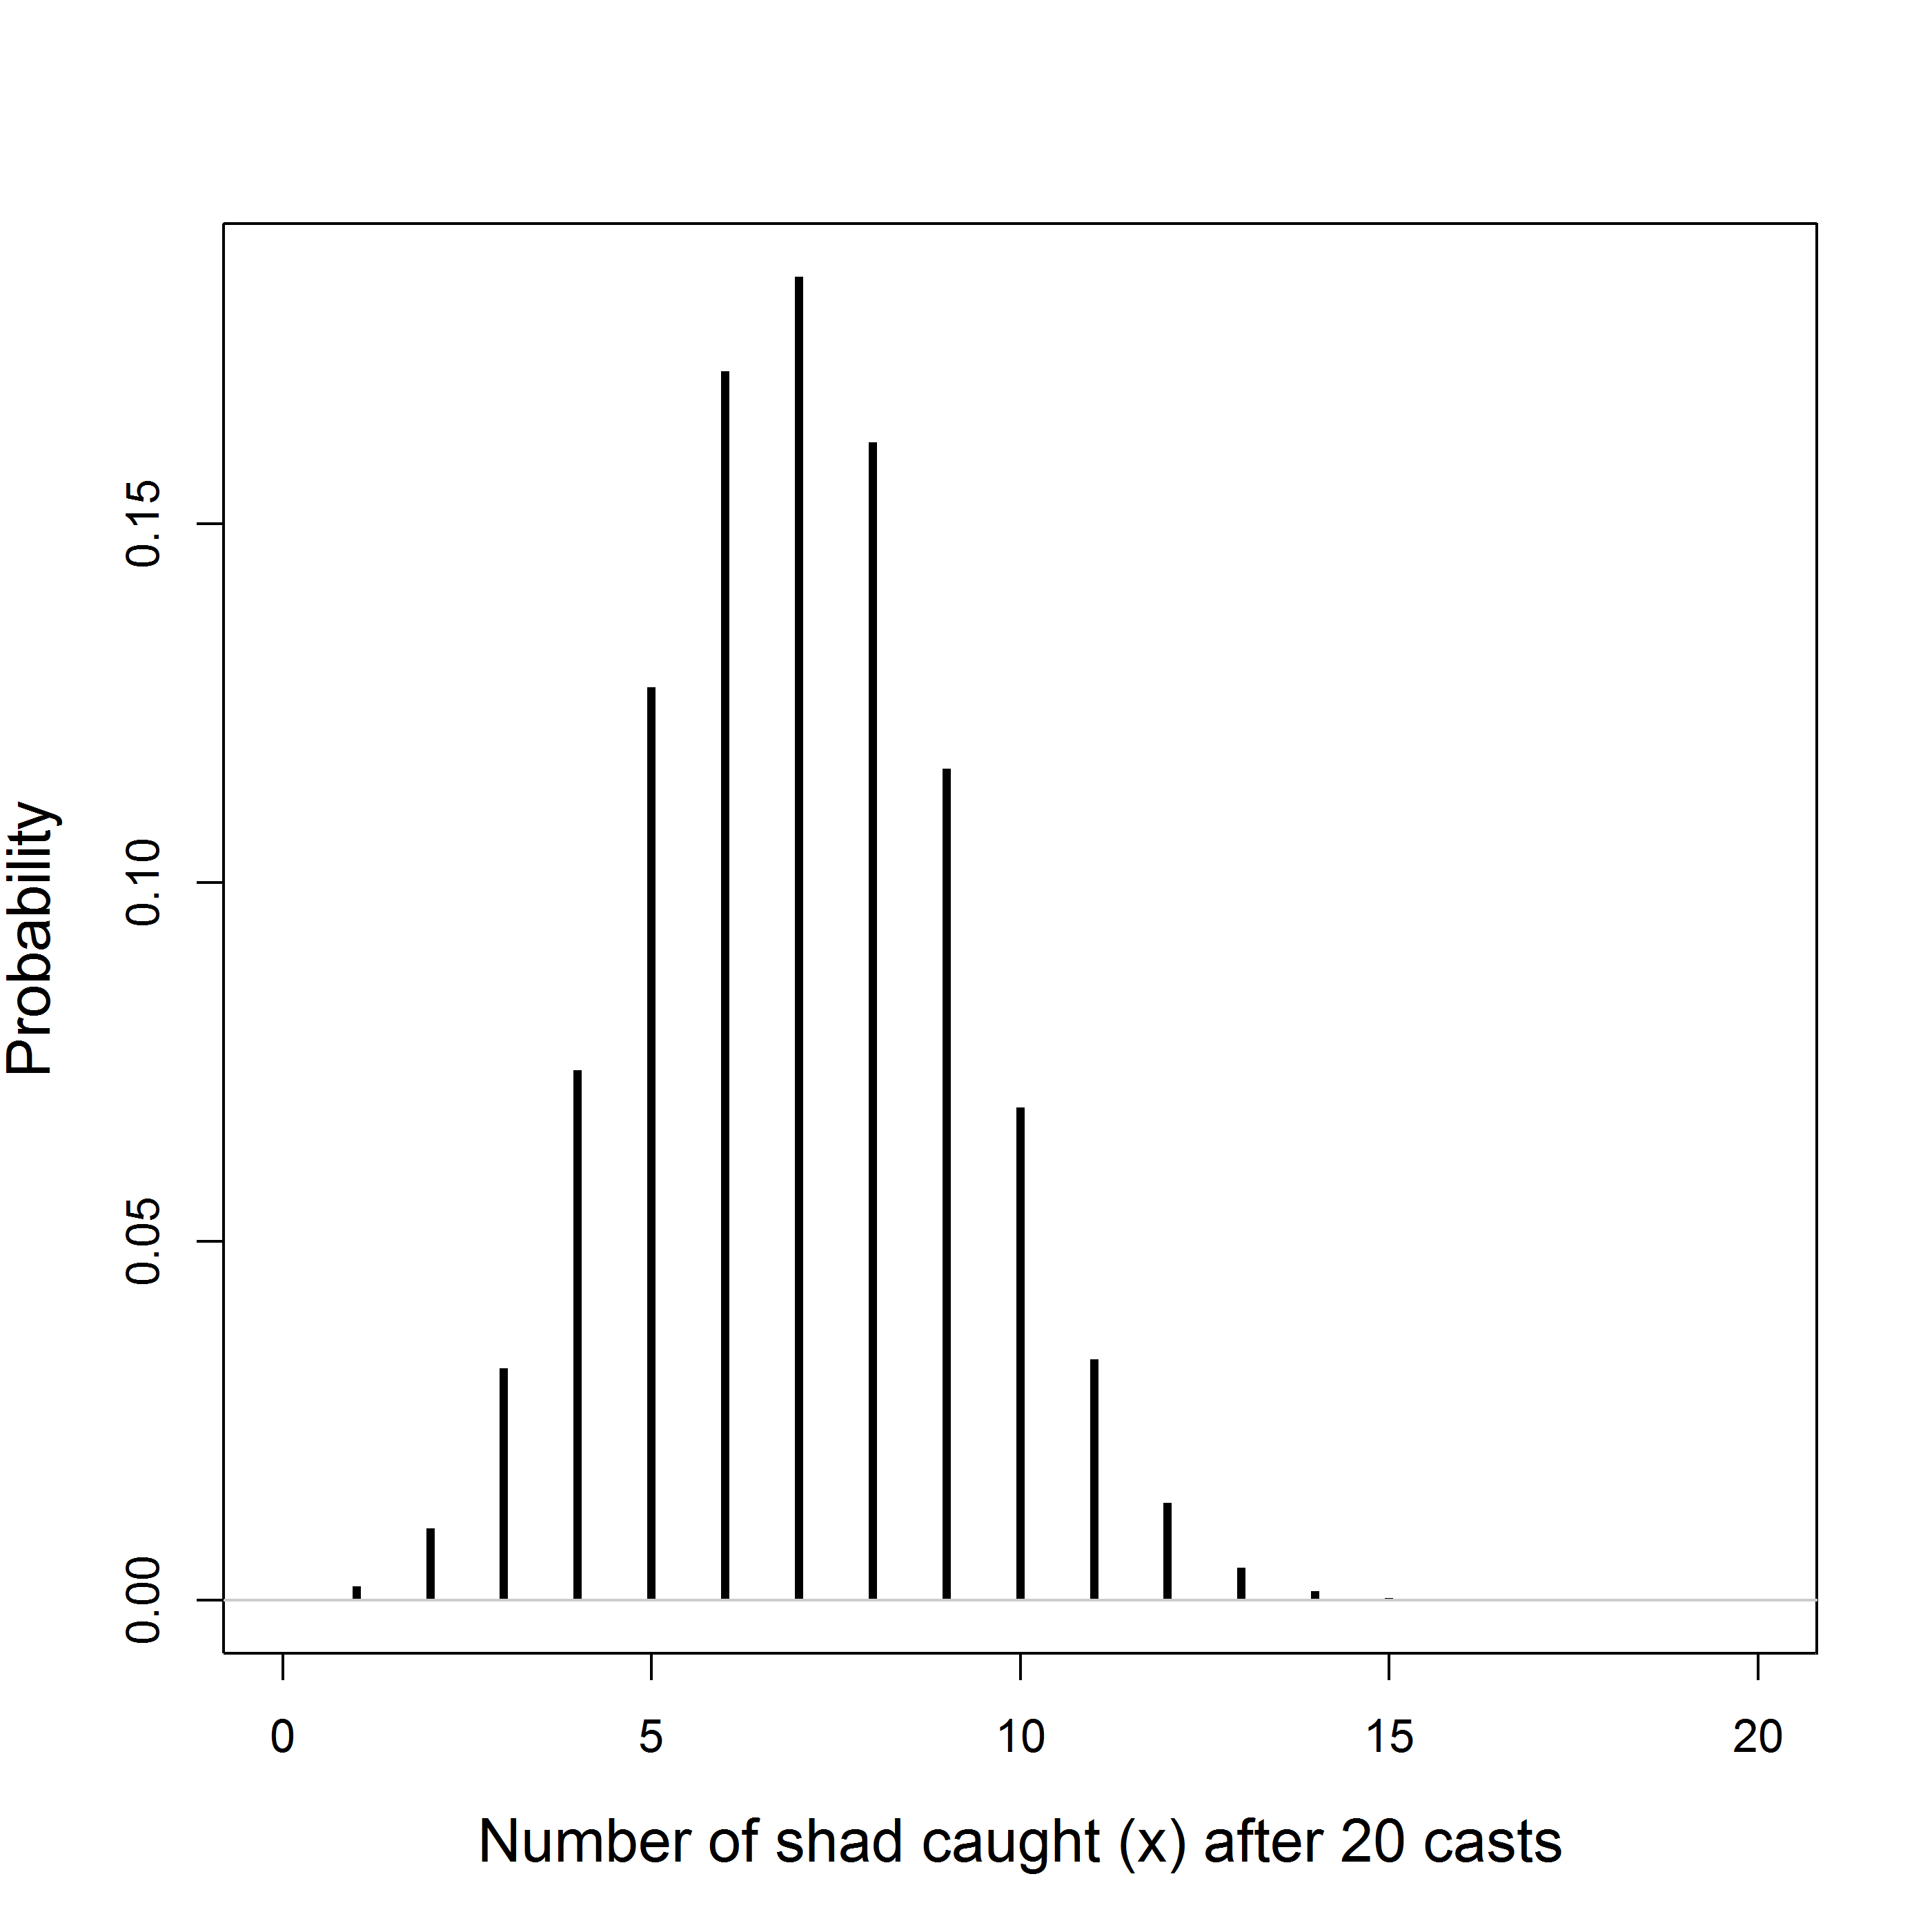
\includegraphics[width=4in,height=4in]{Ch1b/figs/bin}
\caption{The binomial probability mass function with $N=20$ and
  $p=0.35$. }
\label{modeling.fig.bin}
\end{figure}

The purpose of this little example is to show that once we specify a
model for the random variable(s) being studied, we can begin drawing
conclusions, i.e making inferences, about the processes of interest,
even in the face of uncertainty.
Probability distributions are
essential to this process, and thus we need to
understand them in some more depth.


%%%% Add support??
\begin{table}[t!]
  \small
  \caption{Common probability density functions (pdfs) and probability
    mass functions (pmfs) used throughout this book.}
  \begin{tabular}[t]{lcccc}
    \hline
    Distribution & Notation & pdf/pmf & Mean & Variance \\
    \hline
    \multicolumn{5}{c}{Discrete random variables} \\
    Poisson & $x \sim \text{Pois}(\lambda)$ &
    $\exp(-\lambda )\lambda^x/x!$ & $\lambda$ & $\lambda$ \\
    Bernoulli & $x \sim \text{Bern}(p)$ & $p^x(1-p)^{1-x}$ & $p$ &
    $p(1-p)$  \\
    Binomial & x $\sim \text{Bin}(N, p)$ & $\binom{x}{N}p^x(1-p)^{N-x}$
    & $Np$ & $Np(1-p)$  \\
    Multinomial & $\mathbf{x} \sim \text{Multinom}(N, \bm{\pi})$ &
    $\binom{N}{x_1 \cdots x_k}\pi_1^{x_1} \cdots \pi_k^{x_k}$ & $N\pi_k$
    & $N\pi_k(1-\pi_k)$ \\
    \multicolumn{5}{c}{Continuous random variables} \\
    Normal & $x \sim \text{N}(\mu, \sigma^2)$ & $\frac{1}{\sigma\sqrt{2\pi}}
      \exp(-\frac{(x-\mu)^2}{2\sigma^2})$ & $\mu$ & $\sigma^2$  \\
    Uniform & $x \sim \text{Unif}(a, b)$ & $1/(b-a)$ & $(a+b)/2$ &
    $(b-a)^2/12$  \\
%    2D-Uniform & $\mathbf{x} \sim \text{Unif}(\mathcal{S})$ & $1/A(\mathcal{S})$ & &  \\
    Beta & $x \sim \text{Beta}(a, b)$ &
    $\frac{\Gamma(a+b)}{\Gamma(a)+\Gamma(b)}x^{a-1}
    (1-x)^{b-1}$ & $a/(a+b)$ & $\frac{ab}{(a+b)^2(a+b+1)}$ \\
    Gamma & $x \sim \text{Gamma}(a,b)$ &
    $\frac{b^a}{\Gamma(a)}x^{a-1}\exp(-bx)$ & $a/b$ & $a/b^2$  \\
    \hline
  \end{tabular}
  \label{modeling.tab.pdfs}
\end{table}




\subsection{Properties of Probability Distributions}

A pdf or a pfm is a function like any other function
%Probability distributions are functions like any other functions
in the sense that it has one or more arguments whose values determine
the result(s) of the function. However, probability functions have a few
properties that distinguish them from other functions.
The first is that the function
must be non-negative for all possible values of the random variable
$X$, i.e. $[x] \geq 0$. The second requirement is that the integral of
a pdf must be unity, $\int_{-\infty}^{\infty} [x] = 1$, and similarly
for pmf, the summation over all possible values is unity, $\sum_x [x]
= 1$. The following \R~code demonstrates
this for the normal and binomial distributions:
\begin{verbatim}
> integrate(dnorm, -Inf, Inf, mean=0, sd=1)$value
[1] 1
> sum(dbinom(0:5, size=5, p=0.1)) # 5 is as good as Inf here
[1] 1
\end{verbatim}
This requirement is important to remember when one must develop a
non-standard probability distribution. For example, in Chapt.
~\ref{chapt.state-space} and \ref{chapt.rsf},
we work with a resource selection function (RSF) whose probability
density function is not one that is pre-defined in software packages
such as \R~or \bugs.

Another feature of probability distributions is that they can be used
to compute important summaries of random variables. The two most
important summaries are the expected value, $\mathbb{E}(X)$,
and the variance $\text{Var}(X)$. The expected value
can be thought of as the average
value of a very large sample from the specified distribution. For
example, a poor man's way of finding the expected values of a binomial
distribution with $K=20$ trials and $p=0.35$ can be implemented in \R~using:
\begin{verbatim}
> mean(rbinom(10000, 20, 0.3))
[1] 6.9865
\end{verbatim}
For most probability distributions used in this book, the expected
values are known exactly, as shown in Table~\ref{stat.tab.pdfs}, and
thus we don't need to resort to Monte Carlo approximations. For instance, the
expected value of the binomial distribution is $\mathbb{E}[x] = Kp =
20 \times 0.35 = 7$. In this case, it happens to take an integer
value, but this is not a necessary condition, even for discrete random
variables.

A more formal definition of an expected value is the average of all
possible values of the random variable, weighted by their
probabilities. For continuous random variables, this weighted average
is found via integration:
\begin{equation}
  \mathbb{E}(X) = \int_{-\infty}^{\infty} x[x] \, \text{d}{x}.
  \label{modeling:eq:EXc}
\end{equation}
For example, if $[x]$ is normally distributed with mean 3 and unit
variance, we could find the expected value using the following code.
\begin{verbatim}
> integrate(function(x) x*dnorm(x, 3, 1), -Inf, Inf)
3 with absolute error < 0.00033
\end{verbatim}
Of course, the mean \textit{is} the expected values for the normal
distributions, so we didn't need to compute the integral, but the
point is that Eq.~\ref{modeling:eq:EXc} is generic. For discrete
random variables, the expected value is found by summation rather than
integration:
\begin{equation}
  \mathbb{E}(X) = \sum_{x} x[x]
  \label{modeling:eq:EXd}
\end{equation}
where the summation is over all possible values of $x$.

Earlier we
approximted the expected value of the binomial distribution
with $K=20$ trials and $p=0.35$ by taking a Monte Carlo
average. Eq.~\ref{modeling:eq:EXd} let's us
find the exact answer, as done using this bit of \R~code:
\begin{verbatim}
> sum(dbinom(0:100, 20, 0.35)*0:100)
[1] 7
\end{verbatim}
This is great. But of what use is it? One very
important concept to understand is that when we fit (generalized
linear) models, we are modeling the expected value of some random
variable. For example, in Poisson regression, we model $\lambda$, the
expected value of a Poisson random variable, which may be a function
of environmental variables.

The ability to model the expected value of a random variable gets us
very far, but we also need a model for the variance of the random
variable. The variance %is itself a type of expected value; one that
describes the amount of variation around the expected
value. Specifically, $\text{Var}(X) = \mathbb{E}((X -
\mathbb{E}(X))^2)$. Clearly, if the variance is zero, the variable is
not random.

For some distributions, notably the normal distribution, the variance
is a parameter to be estimated. Thus, in ordinary linear regression,
we estimate both the mean (expected value) of the random variable
$\mu$ (which may be a function of covariates) and the variance
$\sigma^2$, or similarly the residual standard error $\sigma$. For
other distributions, the variance is not an explicit parameter to be
estiamted, and instead, the mean to variance ratio is fixed. In the
case of the Poisson distribution, the mean is equal to the
variance, $\mathbb{E}(X) = \text{Var}(X) = \lambda$. This is often viewed as a restriction because in ecology
count data often have a variance greater than the mean. However, much
of this variation can be ``explained'' by modeling the mean as a
function of covarites. Still, in cases where extra-Poisson variation
exists, other distributions such as the negative binomial or
zero-inflated Poisson distribution may be required. A similar
situation is true for the binomial distribuiton---the variance is
determined by the two parameters $K$ and $p$, $\text{Var}(X) = Kp(1-p)$. Thus
in our earlier example with $K=20$ and $p=0.35$, the variance is
4.55. Toying around with these ideas using random number generators
may be helpful. Here is some code
\begin{verbatim}
> 20*0.35*(1-0.35)             # Var(X)
[1] 4.55
> x <- rbinom(100000, 20, 0.35)
> mean((x-mean(x))^2)          # Monte Carlo approximation
[1] 4.545525
\end{verbatim}



\section{Common Probability Distributions}
\label{sec.modeling.distributions}

We got a little ahead of ourselves in the previous example by using
the binomial and Poisson distributions without fully describing them.
A solid understanding of the binomial, Poisson, multinomial, uniform,
and normal distributions is absolutely essential throughout the
remainder of the book. We will occasionally make use of other
distributions such as the beta, log-normal, multivariate-normal,
gamma, Dirichlet, etc... that can be helpful when
modeling capture-recapture data, but these distributions can be
readily understood once you are comfortable with the more commonly
used distributions described in this section.

\subsection{The Binomial Distribution}

We have already briefly introduced the binomial distribution, but we
need to describe it in more detail because of the critical role it
plays in ecology. The binomial distribution is
used for purposes as diverse as modeling count data, survival
probability, occurrence probability, and capture probability.

To describe the properties of the binomial distribution, and related
distributions, we will introduce a new example.
Suppose we are conducting a bird survey at a site in which 10
chestnut-sided warblers (\textit{Stetophaga pensylvanica}) occur and
each of these individuals has a detection probability of 0.5. The
binomial distribution is the natural choice for describing the number
of individuals that we would expect to detect in this
situation, and using our notation, we can write
$x \sim \text{Bin}(10, 0.5)$. Note that if $p \equiv 1$, the number of
individuals that we would observe on $J$ replicate surveys, $x_j$,
would not be a random variable---we would always observe
$x_j=10$. That is the observed data would exactly equal the expected
value and the variance would be zero.
\begin{comment}
  The \texttt{stats} package that comes with \R~has random number
  generators for most of the distributions we will use in this
  book. These functions always begin with \texttt{r}, as in
  \texttt{rbinom} for generating random binomial outcomes. Thus, to
\end{comment}
However, when $p<1$, we can expect that we will observe different
a different number of warblers on each replicate visit. To see this,
we can simulate data under this simple model in which $J=3$ visits are
made to the site:
\begin{verbatim}
> n <- rbinom(3, size=10, prob=0.5)
> n
[1] 6 4 8
\end{verbatim}
The vector $\mathbf{x}$ will typically differ each time you issue this
command; however, we know the probability of observing any value of
$n_j$ because it is defined by the binomial pmf. As we demonstrated
earlier, in \R~this probability can be found using the \verb+dbinom+
function. For example, the probability of observing $n_j=5$ is given by:
\begin{comment}
  Without knowing a thing about probability distributions, most people
  would recognize that the expected value of $x_j$ is $10 \times 0.5 =
  5$. That is, the most likely number of chestnut-sided warblers that
  we would expect to detect is 5. In this case, however, we did not
  observe a single 5, but rather observed counts of 6, 4, and 8
  chestnut-sided warblers on the first, second, and third surveys
  respectively. If 5 is the most likely outcome, how likely was it to
  observe these data? And what is the actual probability of observing
  a 5? These questions can all be answered by the probability mass
  function (pmf) for the binomial distribution.

  The probability of
  observing a 5 (or any other number) when $N=10$ and $p=0.5$ can be
  computed in \R~by issue the following command:
\end{comment}
\begin{verbatim}
dbinom(5, 10, 0.5)
\end{verbatim}
This simply evaluates the function shown in
Table~\ref{stat.tab.pdfs}. We could do the same more transparently, but
less efficiently, using any of the following:
\begin{verbatim}
N <- 10
n <- 5
p <- 0.5
factorial(N)/(factorial(n)*factorial(N-n))*p^n*(1-p)^(N-n)
exp(lgamma(N+1) - (lgamma(n+1) + lgamma(N-n+1)))*p^n*(1-p)^(N-n)
choose(N, n)*p^n*(1-p)^(N-n)
\end{verbatim}

Note that these three expressions differ only in how they compute the
binomial coefficient $\binom{N}{n}$, which is the number of different ways
we could observer 5 of the 10 chestnut-sided warblers at the site. The
binomial coefficient, which is read ``N choose n'' is defined as
\begin{equation}
  \label{eq:1}
  \binom{N}{n} = \frac{N!}{n!(N-n)!}
\end{equation}


\begin{comment}
Now that we know how to compute the probability of observing $n=5$ under
our model, we can compute the probability of observing any
integer $n$ and this allows us to easily visualize the
probability mass function as we did earlier.
  The following command produces a plot of the binomial pmf for
  integers 0 through 15. Notice that the probability of observing
  $n>N$ is zero.

\begin{verbatim}
plot(0:15, dbinom(0:15, 10, 0.5), type="h", lwd=5, lend="butt",
     xlab="n", ylab="Pr(n=x|N,p)")
\end{verbatim}

  In our example, we only drew 3 samples from the binomial
  distribution and it should be evident that it would be difficult to
  estimate parameters of the distribution with such a small
  sample. With a large sample, a histogram of the observed counts
  should closely mimic the true probability mass function as is shown
  here:


  This example illustrates the uncertainty inherent in sampling and
  the


  If our interest was in estimating $N$, and we somehow knew that
  $p=0.5$, our best guess would be that $N$ is the mean of the counts
  divided by the detection probability,
  \[
  \hat{N} = \frac{\mathbb{E}(x)}{p} = \frac{1/J \sum_j x_j}{p} =
  \frac{6}{0.5} = 12.
  \]
  Our estimate is 2 chestnut-sided warblers too high. Not too bad
  though. As it turns out, estimating the binomial $N$ can be quite a
  challenge, which we will discuss in more in the next section on
  estimation. For the moment, it is important to recognize what the
  binomial distribution is, and how it can be used to describe our
  hypotheses about an ecological processs. It also , however, that we
  had nothing better to do than visit the site 100 times. In this
  case, we would expect to observe counts such as this:
\end{comment}



\subsection{The Bernoulli Distribution}

Above, we showed three alternatives to \verb+dbinom+ for evaluating the
binmial pmf. These three commands differed only in how they computed
the binomial coefficient, which we needed because of the numerous ways
in which we could observe $n=5$ under our model. To conceptualize
this, let $h_i$ be the binary variable indicating if individual $i$
was detected or not.
For example, we could observed $\mathbf{h}=(0,0,1,1,1,1,1,0,0,0)$
which is to say that we detected individuals 3-7 but not 1-2 or
8-10. For $N=10$ and $n=5$, there
are 252 possiblities of $\mathbf{h}$. However, when $N \equiv 1$, this term
drops from the pmf and the result is the pmf for the Bernoulli
distribution. That is, the Bernoulli distribution is simply the
binomial distribution when $N \equiv 1$. Alternatively, we could say that the binomial
distribution is the outcome of $N$ i.i.d. Bernoulli trials.

The utility of the Bernoulli distribution is evident when we imagine
that not all of the chestnut-sided warblers have the same detection
probability. Thus, if some individuals can be detected with
probability 0.3 and others have a 0.7 detection probabilty, we can no
longer safely write $n \sim \text{Bin}(N, p)$ since $p$ is no
longer a constant (scalar). %\footnote{Although this model is not
%  technically accurate, it is often a good approximation if
%  heterogeneity in $p$ is low.}.

To properly account for variation in $p$, we could redefine our notation
describing how the counts of chestnut-sided warblers are
generated. Our model now is
\begin{gather}
h_{ij} \sim \text{Bern}(p_i) \quad \text{for} \; i=1,2,\dots,N \\
x_j = \sum_i h_{ij}
\label{modeling.eq.Bern}
\end{gather}

Note that the individual-specific data $h_{ij}$ can observed be
observed when we can keep track of each individual, such as when they
are marked or otherwise distinguishable. In such cases,
the Bernoulli distribution allows us to
model variation in detection probability among individuals and thus
would be preferable to the binomial distribution, we assumes that each
of the $N$ individuals have the same $p$.
For this reason, the Bernoulli
distribution, as simple as it is, is of paramount importance in
capture-recapture models, including spatial capture-recapture models
in which there is virtually always variation in capture probability
among individuals. Indeed, it could be said the Bernoulli model is the
canonical model in capture-recapture studies---most of the
variations in capture-recapture models lie in how $p_i$ is specified,
and how $N$ is estimated.

The Bernoulli pmf is simply $p^n(1-p)^{1-n}$ and hence we do not need canned
functions to facilitate its evaluation. Of course, if you wanted to, you
could always use \verb+dbinom+ with the \verb+size+ argument set to
1.

\subsection{The Multinomial Distribution}


Earlier we let $h_{ij}$ denote a binary variable indicating if
warbler $i$ was detected on survey $j$. The vector of observations for an
individual, $\mathbf{h}_i$, is often referred to as the individual's
``encounter history''. The number of possible encounter
histories depends on the number of survey occasssions. Specifically,
there are $2^J$
possible encounter histories\footnote{When $N$ is unknown, we can
  never observer the encounter history of an individual that is not
  detected, and thus the number of ``observable'' encounter histories
  is $2^(J-1)$}.
If we tabulate the number of individuals with each encounter history,
the frequencies can be modeled using the multinomial
distribution.

The multinomial distribution can be thought of as a
model for placing $N$ items in $K$
categories, which we will also refer to as bins or cells. Each bin has
its own probability $\pi_k$ and
these probabilities must sum to one.
In ecology, $N$ is often population size or the number of individuals
detected, but the definition of the $K$ bins varies among
applications. In standard capture-recapture models, the bins are the
capture histories and the cell probabilities are the probabilities of
observing each capture history. In
distance sampling, when the distance data are in discrete intervals,
the bins are the distance intervals, and the cell probabilities are
the probability of detection in each interval.

Going back to our
chestnut-sided warbler example, suppose the 10 individuals are marked
and we make $J=2$ visits to the site such that there are $2^J = 4$ possible encounter
histories $\mathbf{h} \in c(11, 10, 01, 00)$. If $p=1$, then the
encounter history for each of the 10 individuals would be $11$. That
is, we would detect each individual on both occasions. In this case,
we could format our data as $\mathbf{h} = (10, 0, 0, 0)$. The
cooresponding cell probabilities would be $\bm{\pi} = (1, 0, 0,
0)$. What about the situation where $p<1$, e.g. $p=0.3$? In this case, the
probability of observing the capture history ``11'' (detected on both
occasions) is $pp = 0.3 \times 0.3 = 0.09$. The probability of
observing $10$ is $p*(1-p) = 0.21$. Following this logic, the vector
of cell probabilies is $\bm{\pi} = (0.09, 0.21, 0.21, 0.49)$. We can
simulate data under this model as follows:
\begin{verbatim}
> caphist.probs <- c("11"=0.09, "10"=0.21, "01"=0.21, "00"=0.49)
> drop(rmultinom(1, 10, caphist.probs))
11 10 01 00
 0  3  2  5
\end{verbatim}\footnote{The \verb+drop+ function simply converts the matrix to a vector.}
The
result of our simulation is that zero individuals were observed with
the capture history ``11'' and 5 individuals were observed with the
capture history ``00''. The other 5 individuals were observed one out
of the two occasions. This is not such a surprising outcome given
$p=0.3$. Note that the a single outcome of a multinomial distribution
is a vector, and hence it is a multivariate distribution in contrast
to the univariate distributions discussed so far.

As in non-spatial capture-recapture studies, the multinomial
distribution turns out to be very important in spatial
capture-recapture studies. However, $N$ is typically not population
size. Rather, we use the multinomial distribution when an individual
can only be captured in a single trap during an occasion. Thus, in
this case, $N=1$ and the cell probabilities are the probabilities of
being captured in each trap.

It is worth noting that, just as the Bernoulli distribution is a specific case of the binomial
distribution when $N \equiv 1$, the categorical distribution is a very
similar to a multinomial distribution with size parameter
$N\equiv1$. The only difference is that, rather than returning a
vector with a single element equal to 1, it returns the element number
where the 1 occurs. For example, if $h=(0,0,1,0)$ is an outcome of a
multinomial distribution with $N=1$, then the categorical outcome
would be 3 because the third cell is 1. Thus, in spatial
capture-recapture models, we might use either the multinomial
distribution with $N=1$, or we can just as well use the categorical
distribution. They are equivalent.


\subsection{The Poisson Distribution}

One of the most important models for describing the distribution
of individuals in space is the Poisson point
process. If $N$ individuals are uniformly distributed in some region
$\mathcal{S}$ with area $A$, and $N$ is a
random variable, we call this the homogeneous Poisson point process
whose intensity parameter is $\lambda = 1/A$. The intensity parameter
is defined as the expected number of points that one would find in an
infinitesimally small area. Often, the intensity parameter is not
constant, but rather it takes on different values for each location
$x$ in the region $\mathcal{S}$. The inhomogeneous Poisson point
process model can be useful in such cases, and typically, the
intensity is modeled as a log-linear function of spatially-referenced
environmental covariates. Thus, rather than $\lambda$, the intensity
parameter is now $\lambda(x)$. Inhomogeneous Poisson point process
models have a long history of applications in forestry, and are now
being increasingly used to model species distributions. They are also
extremely important in spatial capture-recapture as we will soon see.

Although the Poisson point process model is very powerful when
coordinate data are available, count data are much more prevalent in
ecological studies. Here too the Poisson distribution acts as the
canonical model, and one of the reasons for this is that count data
can be thought of as spatial aggregations of point data.
Indeed, under the homogeneous Poisson point process model,
then the number of individuals occurring in some
region $B \in A$ is Poisson distributed with expectation
$\lambda = N/A$. As before, $\lambda$ might vary among regions, which
may be distinct habitat patches or arbitrarily-defined survey plots or
quadrats. Modeling spatial variation in $\lambda$ is easily done using
Poisson regression, which is a specific type of generalized linear
model.

One feature of the Poisson distribution that is easily criticized is
that it assumes the mean is equal to the variance. blah and blah.

How will we use the Poisson distribution in spatial-capture recapture
models? One of the most common applications is studies in which an
individual can be detected multiple times at a trap during a single
occasion. For example, in camera trapping studies we might obtain
multiple pictures of the same individual during a sampling
occasion. Thus, $\lambda$ in this case would be defined as the
expected number of detections per occasion.



\subsection{The Uniform Distribution}

The poor uniform distribution is perhaps the most boring of
distributions. I mean, come on, there are no parameters to estimate or
model. The only two parameters are the lower and upper endpoints,
which are almost always known. On the bright side, the uniform
distribution is one of the most widely used,
especially among Bayesians who use it to as a ``non-informative''
prior. We will do this very regularly in this book. For example, if we
have a capture probability parameter $p$ that we wish to estimate, but
we have no prior knowledge of what value it may take in the range
[0,1], we will often use the prior $p \sim \text{Unif}(0,1)$. This
simply states that $p$ is equally likely to take on any value between
zero and one.

Another common use of the uniform distribution is as a prior for the
location of points in a plane. Remember the Poisson point process
described previously---well, a simple way to simulate such data is as
follows:
\begin{verbatim}
s
\end{verbatim}
where $\mathbf{s}$ is the two-dimensional vector of
coordinates. We will often represent this model for the point
locations as
\begin{equation}
  s \sim \text{Unif}(\mathcal{S}),
\end{equation}
although, it would be more correct to somehow distiguish this
two-dimensional uniform distribution for the univariate one. That is,
it might be more clear to use notation such as
$s \sim \text{Unif}_2(\mathcal{S})$ instead. However, this is rather
tedious and cumbersome, so we will opt for the former expression.

\subsection{The Normal Distribution}

Ecologists used to model just about everything as normally
distributed. One reason for this is that methods such a linear
regression and $t$-tests were all that were available in many
primitive stats software programs. Another reason why the normal
distribution, also called the Gaussian distribution, is so attractive
is that it allows us to estimate both the mean and variance of a
random variable, and to model explicit models for each. This is really
great, but often random variables are simply not continuous and cannot
take on values between $-\infty$ and $\infty$. Think of
population size... discrete; presence-absence data... discrete;
survival times... continuous but positive, etc...


\subsection{The Beta Distribution}

Many of the parameters of interest in capture-recapture models are
probabilities---think of capture probability or survival
probability. If we think of these parameters as random variables,
as Bayesians do, then we will often describe these distributions using
the beta distribution. The beta distribution is particularly useful as
a prior for such parameters because it allows us to express either a
lack of knowledge or very precise knowledge about a
parameter. Specifically, a $\text{Beta}(1,1)$ distribution is
equivalent to a $\text{Unif}(0, 1)$ distribution. However, unlike the
the uniform distribution, the beta distribution can be used as an
informative prior; for example if published estimates of detection
probability exist.








\section{Parameter Estimation}

If we know the parameters of a model with absolute certainty, then
we can use pdfs and pmf to make direct
probability statements about unknowns such as future outcomes. However, we
almost never know the actual values of parameters, and instead we have
to estimate them. Our inferences must then acknowledge the uncertainty
associated with our imperfect knowledge of the parameters. Doing so is
most often done using one of two approaches to inference, one referred
to as classical inference and the other known as Bayesian
inference. Both types of statistical inference make heavy use of
probability distributions. In the next chapter, we will review some of
the important concepts in Bayesian inference, so here, we will
focus on classical inference.

In classical inference, if our data are distributed according to some
distribution with unknown parameter $\lambda$, then the only
uncertainty that we are concerned with is that attributable
sampling. For instance, we can imagine repeatedly sampling the
population and each time obtaining a different estimate of $\lambda$.




\section{Joint, Marginal, and Conditional Distributions}

So far we have restricted our attention to single random variables.
However, in ecology, we often are interested in multiple random
variables and how they are related. Define $Y$ as a random variable
whose realized values may or may not be independent of $X$. Inference
about these two random variables can be made using the joint,
marginal, or conditional distributions---or, we may make use of all of
them---it depends upon our question being asked. In the case of
discrete random variables, the joint
distribution is the probability that $X$ takes on the value $x$
\textit{and} that $Y$ takes on the value $y$, which is written
$[X=x,Y=y]$. To clarify this concept, let's go back to our previous
example where $X$ was the number of fish caught after 20 casts, which
we said was an independent and identically distributed (i.i.d.)
binomial random variable. Now,
let's suppose that $X$ depends on the random variable $Y$, which is
the number of other fisherman at the hole. Specifically, let's say
that the probability of catching a fish $p$ is related to $X$
according to $\text{logit}(p) = -0.6 + -2y$. Furthermore, let's
make the intuitive assumption that the number of fishermen at the hole
is a Possion random variable with mean $0.6$, i.e. $x \sim
\text{Poisson}(0.6)$. Our model is now fully specified, and so we can
answer the question, ``what is the probability of catching $x$ fish
\textit{and} of there being $y$ a-holes at the hole. This joint
distribution is given by the product of the binomial pmf (with $p$
determined by $y$), and the Poisson pmf with $\lambda=0.6$. The
following \R~code creates the joint distribution.
\begin{verbatim}
> X <- 0:20 # All possible values of X
> Y <- 0:10  # All possible values of Y
> lambda <- 0.6
> p <- plogis(-0.62 + -2*Y) # p as function of Y
> round(p,2)
 [1] 0.35 0.07 0.01 0.00 0.00 0.00 0.00 0.00 0.00 0.00 0.00
> joint <- matrix(NA, length(X), length(Y))
> rownames(joint) <- paste("X=", X, sep="")
> colnames(joint) <- paste("Y=", Y, sep="")
>
> # Joint distribution [X,Y]
> for(i in 1:length(Y)) {
+     joint[,i] <- dbinom(X, 20, p[i]) * dpois(Y[i], lambda)
+ }
> round(joint,2)
      Y=0  Y=1  Y=2  Y=3 Y=4 Y=5 Y=6 Y=7 Y=8 Y=9 Y=10
X=0  0.00 0.08 0.08 0.02   0   0   0   0   0   0    0
X=1  0.00 0.12 0.02 0.00   0   0   0   0   0   0    0
X=2  0.01 0.08 0.00 0.00   0   0   0   0   0   0    0
X=3  0.02 0.04 0.00 0.00   0   0   0   0   0   0    0
X=4  0.04 0.01 0.00 0.00   0   0   0   0   0   0    0
X=5  0.07 0.00 0.00 0.00   0   0   0   0   0   0    0
X=6  0.09 0.00 0.00 0.00   0   0   0   0   0   0    0
X=7  0.10 0.00 0.00 0.00   0   0   0   0   0   0    0
X=8  0.09 0.00 0.00 0.00   0   0   0   0   0   0    0
X=9  0.06 0.00 0.00 0.00   0   0   0   0   0   0    0
X=10 0.04 0.00 0.00 0.00   0   0   0   0   0   0    0
X=11 0.02 0.00 0.00 0.00   0   0   0   0   0   0    0
X=12 0.01 0.00 0.00 0.00   0   0   0   0   0   0    0
X=13 0.00 0.00 0.00 0.00   0   0   0   0   0   0    0
X=14 0.00 0.00 0.00 0.00   0   0   0   0   0   0    0
X=15 0.00 0.00 0.00 0.00   0   0   0   0   0   0    0
X=16 0.00 0.00 0.00 0.00   0   0   0   0   0   0    0
X=17 0.00 0.00 0.00 0.00   0   0   0   0   0   0    0
X=18 0.00 0.00 0.00 0.00   0   0   0   0   0   0    0
X=19 0.00 0.00 0.00 0.00   0   0   0   0   0   0    0
X=20 0.00 0.00 0.00 0.00   0   0   0   0   0   0    0
\end{verbatim}
This matrix tells us the probability of all possible combinations of
$x$ and $y$, and as dicatated by the law of total probability, the sum
of these probabilities is equal to 1.

Perhaps most fisherman don't care about joint distributions. But, a
question that might be asked is ``what is the probability
of catching 1 fish today?'' Well, we know that this depends upon the
number of fisherman, but we don't know how many will show up
today. This brings us to the marginal distribution, which is defined by
\begin{equation*}
  [X] = \sum_Y [X|Y] \qquad
  [Y] = \sum_X [Y|X]
\end{equation*}
for discrete random variables, and
\begin{equation*}
  [X] = \int_{-\infty}^\infty [X|Y] \, \mathrm{d}Y \qquad
  [Y] = \int_{-\infty}^\infty [Y|X] \, \mathrm{d}X
\end{equation*}
for continuous random variables. The key idea here is that to get the
marginal distribution of $X$, we have to contemplate all possible
values of $Y$. Computing marginal distributions is a key step in
maximilizing likelihoods involving random effects, as will be
demonstrated in Chapt.\ref{chapt.mle}. Here is some \R~code to compute
the marginal distribution of $X$, i.e. the probability of $X=x$ fish:
\begin{verbatim}
> margX <- rowSums(joint)
> round(margX, 2)
 X=0  X=1  X=2  X=3  X=4  X=5  X=6  X=7  X=8  X=9 X=10 X=11 X=12 X=13 X=14
0.18 0.14 0.09 0.05 0.05 0.07 0.09 0.10 0.09 0.06 0.04 0.02 0.01 0.00 0.00
X=15 X=16 X=17 X=18 X=19 X=20
0.00 0.00 0.00 0.00 0.00 0.00
\end{verbatim}
Bad news---the most likely value is $X=0$, but there is a simliar
probability of catching 1 fish.

The last type of question we can ask about these two random variables
relates to their conditional distributions. The
conditional probability distribution is the distribution of one
variable, given a realized value of the other. In the case of two discrete random
variables, the conditional distribution may be written as
$[X=x|Y=y]$, i.e. the probability of $X$ taking on the value $x$
given the realized value of $Y$ being $y$. For simplicity, we will
write this as $[X|Y]$. Conditional distributions are defined as follows:
\begin{equation*}
  [X|Y] = \frac{[X,Y]}{[Y]} \qquad [Y|X] = \frac{[X,Y]}{[X]}.
\end{equation*}
That is, the conditional distribution of $X$ given $Y$ is the joint
distbution divided by the marginal distribution of $Y$.
\begin{verbatim}
> XgivenY <- joint/matrix(margY, nrow(joint), ncol(joint), byrow=TRUE)
> round(XgivenY, 2)
      Y=0  Y=1  Y=2  Y=3 Y=4 Y=5 Y=6 Y=7 Y=8 Y=9 Y=10
X=0  0.00 0.25 0.82 0.97   1   1   1   1   1   1    1
X=1  0.00 0.36 0.16 0.03   0   0   0   0   0   0    0
X=2  0.01 0.25 0.02 0.00   0   0   0   0   0   0    0
X=3  0.03 0.11 0.00 0.00   0   0   0   0   0   0    0
X=4  0.07 0.03 0.00 0.00   0   0   0   0   0   0    0
X=5  0.13 0.01 0.00 0.00   0   0   0   0   0   0    0
X=6  0.17 0.00 0.00 0.00   0   0   0   0   0   0    0
X=7  0.18 0.00 0.00 0.00   0   0   0   0   0   0    0
X=8  0.16 0.00 0.00 0.00   0   0   0   0   0   0    0
X=9  0.12 0.00 0.00 0.00   0   0   0   0   0   0    0
X=10 0.07 0.00 0.00 0.00   0   0   0   0   0   0    0
X=11 0.03 0.00 0.00 0.00   0   0   0   0   0   0    0
X=12 0.01 0.00 0.00 0.00   0   0   0   0   0   0    0
X=13 0.00 0.00 0.00 0.00   0   0   0   0   0   0    0
X=14 0.00 0.00 0.00 0.00   0   0   0   0   0   0    0
X=15 0.00 0.00 0.00 0.00   0   0   0   0   0   0    0
X=16 0.00 0.00 0.00 0.00   0   0   0   0   0   0    0
X=17 0.00 0.00 0.00 0.00   0   0   0   0   0   0    0
X=18 0.00 0.00 0.00 0.00   0   0   0   0   0   0    0
X=19 0.00 0.00 0.00 0.00   0   0   0   0   0   0    0
X=20 0.00 0.00 0.00 0.00   0   0   0   0   0   0    0
\end{verbatim}
Note that we have 11 probability distributions for $X$, one for each
possible value of $Y$, and each pmf sums to unity as it should. Note
also that if you show up at the hole and there are more than 2
fisherman, you might want to head home (assuming you actually want to
catch a fish).
%Why is this? Well, remember that capture probability
%declined as a function of the the number of fisherman.

These concepts are explained in more detail, and with more attention
to detail, in other texts such as \citet{casella_burger:2001}, but hopefully, the
code shown here complements the equations and makes it easier for
non-statisticians to understand these concepts.

The last point we wish
to make in the section is that this simple toy example is an example
of a hierarchical model, and we can put all the pieces together using
the following notation:
\begin{gather}
  y \sim \text{Poisson}(0.6) \\
  \text{logit}(p_y) = -0.6 + -2y \\
  x|y \sim \text{Binomial}(20, p_y)
\end{gather}
From here on out, when you see such notation, you should immediately
grasp the fact that $y$ is a random variable independent of $x$, but
$x$ depends upon $y$ through $p$. Now you have the tools to make
probability statements about the random variables in this system. The
one caveat faced in reality is that we typically do not know the
values of the parameters, and instead we have to estimate them.[DETAILS]









\section{Hierarchical Models and Inference}

The term hierarchical modeling (or hierarchical model) has become
something of a buzzword over the last decade with hundreds of papers
published in ecological journals using that term.  So then, what
exactly is a hierarchical model, anyhow? Obviously, this term stems
from the root ``hierarchy'' which means:

\vspace{.1in}

{\flushleft
Definition: {\it hierarchy} (noun) -- a series of ordered groupings of people or things within a system;
}

\vspace{.1in}

In the case of a hierarchical model (hierarchical being the adjective
form of hierarchy), the ``things'' are probability distributions, and
they are ordered according to their conditional probability structure.
Thus, a hierarchical model is {\it an ordered series of models,
  ordered by their conditional probability structure}.

If we declare that the random variable $y = $ \# of times an
individual is encountered in a trap out of $K=10$ days has a
$\mbox{Bin}(10, p)$ distribution then this is but a single model and,
thus, not a hierarchical model. If, however, we declare that
\[
y \sim \mbox{Bin}(10,p)
\]
{\it and}
\[
p \sim \mbox{beta}(1,1)
\]
which is the same as the previous model but with a ``flat'' prior
distribution on $p$, then this is kind of a cheap pedestrian
hierarchical model according to our definition although it is barely
more interesting than the previous non-hierarchical model.
%% I think here in the intro you could remove this 'pedestrian hierarchical model'
%% For the readers who are not familiar (yet) with distributions and what a prior is, I think it would be mroe helpful
%% to only use the following example and explain briefly what the
%% p_{i}\sim \mbox{beta}(\mu, \tau) stands for
On the
other hand, suppose we have some meaningful group structure in this
problem such that the data arise by observing repeated Bernoulli
trials on {\it individuals}, e.g., they are eggs hatching from a
common nest (or parentage). So let $y_{i}$ be the outcomes for
individuals $i=1,2,...,N$ with
\[
y_{i} \sim \mbox{Bin}(K, p_{i})
\]
 and
\[
p_{i}\sim \mbox{beta}(\mu, \tau).
\]
Because of the meaningful group structure, this is a more interesting
hierarchical model. In fact, in the context of capture-recapture this
is a specific version of ``Model Mh'' (see Chapt. 3 and
\citet{dorazio_royle:2003}).  We should consider this a type of a
hierarchical model although we will make a further conceptual
distinction shortly that further dichotimizes the space of
hierarchical models.

A canonical hierarchical model in ecology is this
elemental model of species occurrence or distribution
\citep{mackenzie_etal:2002, tyre_etal:2003, kery:2011}:
\[
y_{i}|z_{i} \sim \mbox{Bin}(K,z_{i} \,  p)
\]
\[
z_{i} \sim \mbox{Bern}(\psi)
\]
where  $y_{i} = $ observation of presence/absence at a site $i$ and
$z_{i} = $ occurrence status ($z_{i}=1$ if a species occurs at  site
$i$ and $z_{i}=0$ if not).  This model has an important conceptual
distinction between the hierarchical model shown just previously
(Model Mh) and also other types of classical multi-level models such
as repeated measures on subjects, in that $z_{i}$ is an actual state
of nature. In that sense, $z$ is a random variable that is the outcome of a
``real'' process.   \citet{royle_dorazio:2008} used the term {\it
  explicit} hierarchical model to describe this type of model to
distinguish from hierarchical models ({\it implicit} hierarchical
models) where the latent variables don't
correspond to an actual state of nature -- but rather just soak up
variation that is unmodeled by explicit elements of the model.
At best, latent variables in such models
are a a surrogate for something of ecological relevance
(``time effects'', ``space effects'' etc.).


With these examples,
we expand on our definition of a hierarchical model as we will use it
in this book: \newline
{\flushleft {\bf Definition}: {\it Hierarchical Model}: A model with
  explicit component models that describe variation in the data due to
  (spatial/temporal) variation in {\it ecological process}, and due to
  {\it imperfect observation} of the process.
}



%\subsection{Anatomy of a hierarchical model}
%Interesting hierarchical models in ecology typically
%contain the following components:
%\begin{itemize}
%\item[{\bf 1.}] {\it Observations}, $y(s,t)$ -- ``data''
%\item[{\bf 2.}] {\it Observation model} $[y|z,\theta_1]$
%\item[{\bf 3.}] {\it State variable}, $z(s,t)$: outcome of ecological {\it process} of interest
%\item[{\bf 4.}] {\it Process model}  $[z|\theta_2]$
%\item[{\bf 5.}] {\it Parameters}, $\theta_1$, $\theta_2$, that govern
%  the observation and state processes
%\end{itemize}


\subsection{Spatial Capture-Recapture models as hierarchical models}

Most models considered in this book describe the encounter of
individuals conditional on the ``activity center'' of the individual,
which is a latent variable (i.e., unobserved random effect).  The
collection of these latent variables represents the outcome of an
ecological process describing how individuals distribute themselves
over the landscape. Moreover, how individuals are encountered in traps
is, in some cases, the result of a model governing movement.  As such,
these models are examples of hierarchical models that contain formal
model components representing both ecological process and also the
observation of that process. That is, they are explicit hierarchical
models \citep{royle_dorazio:2008} as opposed to implicit hierarchical
models.




\section{Characterization of SCR models}
\label{intro.sec.characterization}

For the purposes of this book, an SCR model is any ``individual
encounter model'' (not just ``capture-recapture''!) where auxiliary
spatial information is also obtained. To be more precise we could as
well use the term ``Spatial capture and/or recapture'' but that is
slightly unwieldy and, besides, it also abbreviates to SCR. The class
of SCR models includes traditional capture-recapture models with
auxiliary spatial information and even some
models that do not even require ``recapture'' (e.g., distance
sampling).  There is even a class of models (Chapt. \ref{chapt.scr-unmarked})
which don't require unique capture or
identification of individuals.

Conceptually SCR models involve a collection of random
variables, ${\bf s}$, ${\bf u}$ and $y$ where ${\bf s}$ are the
activity or home range centers, ${\bf u}$ is the location of the
individual at the time of sampling (i.e., where the observer records
the animal) which we think of as realizations from some movement
model, and $y$ is the ``response variable'' - what the observer
records. E.g., $y=1$ means ``detected'' and $y=0$ means ``not
detected'' but many other types of responses are possible.
A broad class of models for estimating density are unified by a
hierarchical model involving explicit models for
animal home range centers ${\bf s}$, movement outcomes ${\bf u}$, and
encounter data $y$.  In some cases, we don't observe $y$ but rather
summaries of $y$, say $n(y)$, yet it might be convenient in such cases
to retain an explicit focus on $y$ in terms of model construction.
We thus introduce a sequence of models - a hierarchical model -
to relate these random variables and it goes something like this:
{\small
\begin{verbatim}
# NEED A graphic made out of this somehow
# possibly a Directed Acyclic Graph with some parameters,
# Fixed nodes, and stochastic nodes, might look cool.

Home range center    movement model   observation model  [data summarization]
   g(s)                  h(u|s)            f(y|u)	        n(y)
\end{verbatim}
}
Thus, models covered in this book all have distinct
characteristics related to the following decomposition as a
hierarchical model:
\[
f(y|{\bf u})h({\bf u}|{\bf s})g({\bf s}).
\]

Every model we talk about in this book has either all of these
components or a subset of them. Fig.\ref{intro.fig.fig1} is an example of the whole
enchilada in which we make the following assumptions:
\begin{gather}
{\bf s}_{i} \sim \mbox{Uniform}({\cal S}) \\
{\bf u}_{ik} | {\bf s}_{i} \sim \mbox{Normal}({\bf s}_{i}, \sigma) \\
y_{ijk} | {\bf u}_{ik} \sim \mbox{Bernoulli}(p(\| x_j - u_{ik} \|)
\end{gather}
These ``assumptions'' are statistical statements of three basic hypotheses
that (1) activity centers are uniformly distributed in two-dimensional
space, (2) movements are normally distributed around the activity
centers, and (3) capture probability is a funciton of the distance
between the animal and the trap. Each of thse model components can be
modified as need to match specific hypotheses, study designs, and data
structures.

\begin{comment}

{\small
\begin{verbatim}
set.seed(36372)       # so that results can be reproduced
N <- 10               # population size
                      # create trap coordinates:
x <- cbind(rep(seq(0.1,0.9,0.2), each=5), rep(seq(0.1,0.9,0.2), times=5))
                      # generate individual home range centroids
s <- cbind(runif(N), runif(N))
                      # create nice graphic:
plot(x, pch= "+", xlim=c(0,1), ylim=c(0,1), xlab="Easting", ylab="Northing")
points(s, pch=16, col="blue")
for(t in 1:5) {
  points(cbind(rnorm(N, s[,1], 0.05), rnorm(N, s[,2], 0.05)), col="green",pch=20)
}
\end{verbatim}
}

\end{comment}

Fig. \ref{intro.fig.fig1} shows the results of executing these {\bf R} commands. The crosses
in the figure are trap locations, the blue circles are the locations
of each animal's activity center, and the green circles are animal
locations at 5 points in time.  The resulting plot not only
illustrates a simple state model for animal distribution and movement,
but it also hints at the potential influence of the distance between
animals and traps on the detection process. One would expect that the
traps in the northern part of the study area would capture more
animals than those in the south because fewer animals occur in the
south and movements are small. Clearly the encounter rate will also
depend upon the methods used to capture the animals, which we describe
in the next section.  Spatial capture-recapture models provide a
statistical formalization of these considerations.


\begin{figure}
\begin{center}
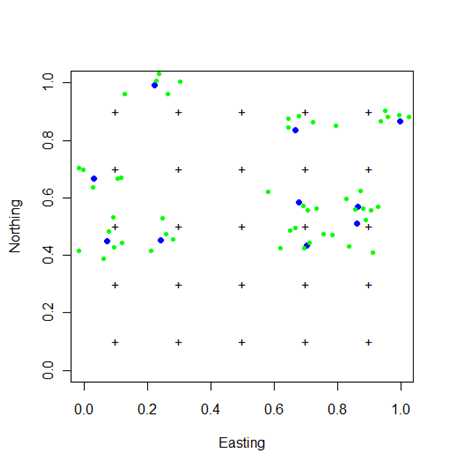
\includegraphics[height=3in]{Ch1/figs/northingeasting}
\end{center}
\caption{Population of $N$ individual home-range centers ($\bf s_i$,
  blue points) and locations during $K=5$ occasions ($\bf u_{ik}$,
  black points). Crosses represent trap locations.}
\label{intro.fig.fig1}
\end{figure}



Although the full model including $u$ and $s$ fully describes the
ecological process, in practice we usually work with reduced forms of
this model. Examples include:
of such models are:
\begin{enumerate}
\item[$\bullet$] Classical distance sampling
\item[$\bullet$] Spatial capture-recapture models with fixed arrays of traps
  \citep{efford:2004, borchers_efford:2008, royle_etal:2009ecol,
    royle_etal:2009jae, gardner_etal:2010ecol,royle_etal:2011jwm}
\item[$\bullet$] Search-encounter models \citep{royle_young:2008, royle_etal:2011mee}.
\item[$\bullet$] Capture-recapture distance-sampling \citep{borchers_etal:1998}.
\end{enumerate}
In some classes of models, components for ${\bf u}$ and ${\bf s}$ will be confounded.
e.g., if ${\bf s}$ are uniform in space and ${\bf u}$ is
a random draw from some distribution centered at ${\bf s}$, then we might as
well define ${\bf u}^{*}=\Pr({\bf u})=\int_{s} [{\bf u}|{\bf s}][{\bf
  s}]ds$ which will itself by uniform
for reasonable choices of $[{\bf u}|{\bf s}]$.  Some examples
of typical spatial capture-recapture models and how
these various model components are manifest in specific cases is
described as follows:
\begin{itemize}
\item[1.] {\bf Distance sampling -- } The last 2 stages of the hierarchy
  are confounded (implicitly) and so analysis is based on the model
  $[y|u*] [u*]$. The ``process model'' is that of ``uniformity'': ${\bf u}^{*}
  \sim Unif({\cal S})$. Sometimes it is argued that distance sampling
  estimators are ``pooling robust'' which is a way of saying they are
  (or may be)
  relatively insensitive to this assumption. That may be true, but the
  construction of distance sampling estimators makes explicit the
  uniformity assumption as a mathematical fact.

\item[2.] {\bf Spatial capture-recapture model with a fixed array of traps} --
SCR models appear to have little in common with distance sampling
because observations are made only at a pre-defined set of discrete
locations -- where traps are placed. However, the models are closely
related in terms of our hierarchical representation above\footnote{Really
they're kind of like point-count distance sampling where the identity
of individuals is preserved across point samples , and distance is a
latent variable. i.e., SCR-DS. I feel like this point should be
emphasized somehow. Here? Later?}
In SCR models based on fixed arrays,
we cannot estimate both
$\Pr(y=1|{\bf u})$ and $\Pr({\bf u}|{\bf s})$ -- the probability  that
an individual ``moves to ${\bf u}$'' cannot be seperated from the
probability that it is detected given that it moves to ${\bf u}$,
because of the fact that the observation locations are fixed by
design.
Formally, such SCR models confound $[y|{\bf u}]$  with $[{\bf
  u}|{\bf s}]$ so that the observation model arises as:
\[
 [y|{\bf s}] = \int_{u} [y|{\bf u}][{\bf u}|{\bf s}] du
\]
This confounding happens because SCR sampling is spatially biased -
restricted to a fixed pre-determined set of locations.

Conversely,
distance sampling confounds $[{\bf u}|{\bf s}][{\bf s}]$ because, essentially, there is
only a single realization of the encounter process.

It is probably
reasonable to assume that $\Pr(y=1|{\bf u})=1$ or at least it is locally
constant for most devices (e.g., cameras, etc..), and thus the
detection model will have the interpretation in terms of movement (see
chapter XXX.YY).

\item[3.] {\bf Search-encounter models -- } What we call
  ``search-encounter'' models \citep{royle_etal:2011mee}
  are kind of a hybrid model - combining features of SCR models and
  features of distance sampling. Like distance sampling they allow for
  encounters in continuous space which provide direct observations
  from $[{\bf u}|{\bf s}]$.
Thus, the
  hierarchical model is fully identified.

\item[4.] {\bf Capture-recapture/distance-sampling -- } See
  \citet{borchers_etal:1998}. As with the search-encounter models the
full hierarchical model is identified:
$[y|{\bf u}][{\bf u}|{\bf s}][{\bf s}]$ but the quantities don't
really mean the same thing as before.

To understand this, we expand the model to accommodate imperfect
measurements of ${\bf u}$. Let ${\bf u}_{obs}$ be an observation of
${\bf u}$ (i.e., made with error). A larger hiearchical model is this:
\[
[y|{\bf u}][{\bf u}_{obs}|{\bf u}][{\bf u}|{\bf s}][{\bf s}]
\]
If we make replicate ``instantaneous'' observations of location, then
information is provided about
 $[{\bf u}_{obs}|{\bf u}]$ (i.e., measurement error). However, in a normal
 distance sampling application, with instantaneous sampling, we don't
 learn anything about $[{\bf u}|{\bf s}]$,
in effect, we are again confounding $[{\bf u}|{\bf s}]$ and $[{\bf
  s}]$: ${\bf u}^{*} = \int_{s} [{\bf u}|{\bf s}][{\bf s}] ds$. So the CR-DS model focuses on:
\[
[y|{\bf u}^{*}][{\bf u}_{obs}|{\bf u}^{*}][{\bf u}^{*}].
\]
Structurally, this is the same basic model as the search-encounter
model notwithstanding (1) that it is usually talked about in terms of
repeated measures of distance instead of location and (2) the 2nd
component of the hierarchy is not movement (an ecological process) but
rather ``measurement error'' and (3) the third component is not a home
range center but rather a movement outcome (``instantaneous
location'').  Thus, while the models are structurally identically, the
meaning and interpretation of quantities are distinct.

%These are
%mostly all semantic and conceptual distinctions which are easy to
%define in a convenient table:
%\begin{table}[ht]
%\centering
%\title{What things mean in each model.}
%\begin{tabular}{c|cc}
%           &   Search encounter models     &  CR-DS  \\  \hline
%  $\sigma$    &  movement       &   measurement error  \\
% ${\bf s}$ & activity center & instaneous location \\
%\end{tabular}
%\end{table}
\end{itemize}

Efford's characterization:
proximity detectors, multi-catch, single-catch, etc....
acoustic detectors, ....

\section{Analysis of spatial capture-recapture models}





%\begin{comment}
\subsection{Models don't have political views!}

Whereas hierarchical modeling is a conceptual and framework for
formulating models, the method of inference is independent of model
formulation. Hierarchical models can be analyzed by Bayesian and
non-Bayesian methods. A model is not Bayesian or frequentist -- what
you do to that model is Bayesian or frequentist!
\[
\bullet \mbox{"Hierarchical model"} \ne  \mbox{"Bayesian"}!!!
\]
Thus, analysis of hierarchical models is easily achieved using either
Bayesian or classical (likelihood, frequentist) methods. By
``analysis'' we mean any type of estimation, characterization of
uncertainty, prediction, model selection, or evaluation and we are not
dogmatic about our choice of inference methods. That said, we do
recognize a benefit of the Bayesian approach which is that it
emphasizes model construction and not the construction of
procedures. The Nobel prize\footnote{called something else besides
  Nobel, officially} winning econometrician Christopher Sims (Slides
from the Hotelling Lecture 6/29/2007 at Duke University - cite his
webpage) said it this way: ``Bayesian inference is a way of thinking,
not a basket of 'Methods''' Conversely, ecologistis that are subjected
to a classical statistical curriculum often have only a vague sense of
what the model is that any particular procedure is employing.  We
agree with Little \citet{little:2006}
that there should be more emphasis on understanding statistical
modeling, and less emphasis on statistical methods.  Toss the ``basket
of methods'' out the window and learn how to model!

%\end{comment}

We rely strictly on principles and procedures of {\it parametric
  inference} in our analysis of hierarchical models in general and,
specifically, of spatial capture-recapture models. Parametric
inference is that in which we make explicit probability assumptions
about how the data were generated. Inference procedures are then
developed under the assumption that the model is truth, because formal
parametric inference procedures that we understand the joint
probability distribution of everything that is a realization of a
random variable. {\bf There is something missing in the previous sentence. require, maybe?}There are two popular flavors of parametric
inference: {\bf Classical inference}: The joint probability distribution
of observations is the {\bf likelihood}. We maximize it to obtain MLEs
and do other fun things to it. We evaluate procedures by thinking
about what would happen over replicate realizations of data to which
our procedures are applied.  {\bf Bayesian inference} is based on the
posterior distribution, which is the joint probability distribution of
the data and also parameters and possibly other quantities including
latent variables or random effects.

Because SCR models contain a collection of latent variables - random
effects -- a natural framework for classical analysis of the models is
based on integrated likelihood \citep{laird_ware:1982,berger_etal:1999}. That is, while
the observation model is conceptualized conditional on the random
effects (the locations of individuals), classical inference is
formally based on the likelihood constructed from the {\it marginal}
probability distribution of the observations (i.e., {\it
  unconditional} on the random effect). The random effects are removed
from the conditional likelihood by integration (which is accomplished
numerically in spatial capture-recapture models). This approach to
inference has been formalized in the context of SCR models by
\citet{borchers_efford:2008, efford:2011}, and implemented for some
classes of models in the software package {\bf DENSITY} \citep{efford:2004}
and the {\bf R} package \mbox{\tt secr} \citep{efford:2011}.

Bayesian analysis is another natural framework for the analysis of
models containing latent variables or random effects.  Under this
approach, analysis of the model is based on Monte Carlo simulation
from the posterior distribution, which is the product of the
conditional likelihood, the distribution of the random effects, and
perhaps other distributions.  This approach was developed by
\citet{royle_young:2008}, and was motivated by work focused on
modeling individual effects in capture-recapture models. In
particular, a convenient reparameterization of individual covariate
models can be obtained using a method known as data augmentation
\citep{royle_etal:2007}, see \citet{royle:2008} for an application to
classical individual covariate models in \citet{royle:2008}. The close
similarity between individual covariate models and spatial
capture-recapture models, with the individual's activity center ${\bf
  s}$ being the individual covariate, led to the application of the
data augmentation method described by \citet{royle_young:2008} and subsequent papers.

These two technical formulations (classical inference based on
integrated likelihood and Bayesian inference) both provide rigorous solutions to
the inference problems posed by spatial capture-recapture data.  There
are also minor distinctions to be aware of. For example,
as a technical matter, \citet{borchers_efford:2008} and related work, assume
a Poisson point process that is unconditional on $N$ whereas Royle and
Young (2008) and related work assume a binomial point process model
which is conditional on $N$.
%More importantly, Borchers and Efford
%develop the analysis in a way that is unconditional on the point
%process (which is removed from the conditional likelihood by
%integration).  Conversely, the analysis of \citet{royle_young:2008} is
%conditional on the underlying point process. As a technical matter,
%Bayesian analysis allows us to analyze the model that is conditional
%on the underlying point process and will otherwise have more
%flexibility - open populations, using telemetry data, etc.. as will be
%demonstrated in later chapters.

We tend to favor Bayesian inference for conceptual and philosphical
reasons but we also think that  integrated likelihood
for complex point process models may prove difficult. On the other
hand, we suspect that Bayesian
analysis by MCMC
of the model that is conditional on the underlying point process will
prove to be more versatile and generalizable for complex point process
models. We say this only
tentatively and throughout this book we are not exclusive in our views
of inference and use Bayesian and classical methods of inference
interchangeable and opportunistically in this book.
We don't want to get too much into the technical foundations of
Bayesian analysis because there are many good books now including
\citet{link_barker:2010}.  \citet{kery:2010, mccarthy:2007,
  king_etal:2009} and probably others by the time this book is
finished. That said,  Bayesian analysis is introduced at a
level required to get through this book in Chapter 2.


%\subsection{Implementing hierarchical models}



\subsection{Estimation}


Maximum likelihood: point estimates, var-covar matrix, confidence
intervals

Bayesian: analytical, simulation (MCMC)




\subsection{Modeling covariate effects}

identity, log, logit, cloglog links


Dummy variables





\section{Criticisms of Hierarchical Models}

\hl{If we keep this, remove all SCR references b/c Andy will address
  those in Chapt 5}

We have frequently used the terms
``assumptions'' and ``priors'', which make some people feel
uneasy. Our view is that expressed eloquently by Link (ADD
QUOTE). Furthermore, we note that hierarchical models allow us to
modify any assumption deemed too
restrictive. That is, we can always generalize our models given enough
data. Chapter is a classic example because it addresses
perhaps the most common criticism of SCR, that ``real animals'' don't
have symmetic home ranges. In fact people have written entire papers
beating up on SCR because they \emph{assume} that this the bivariate
normal model for the encounter processes is a rigid requirement of SCR
methods. Although we believe this assumption is quite reasonable in
many contexts, Chapter \ref{chapt.ecoldist} clearly illustrates that
alternatives exist, and that SCR provides a rigours framework for
testing for departures from this assumption, and even evaluating
hypotheses that may explain why animals move the way they do.





\begin{comment}

\chapter{Bayesian GLMS and WinBUGS, etc..}
\label{chapt.glms}

\chapter{Closed population models}
\label{chapt.closed}


\chapter{Fully Spatial Capture-Recapture Models}
\label{chapt.scr0}


\chapter{Other observation models}
\label{chapt.poisson}


\chapter{Maximum likelihood estimation}
\label{chapt.mle}


\chapter{MCMC details}
\label{chapt.mcmc}


\chapter{Goodness of Fit and stuff}
\label{chapt.gof}



\chapter{Covariate models}
\label{chapt.covariates}


\chapter{Inhomogeneous Point Process}
\label{chapt.ipp}

\chapter{Open models}
\label{chapt.open}


\end{comment}


\bibliography{AndyRefs_alphabetized}


\end{document}